% (This started life as a...) Brief report style paper

% It's about how a somatotopically ordered pattern can be
% re-established in the cortex based on information carried with
% thalamocortical axons afferent from the ventrobasal thalamus, but
% without specifying absolute positions as center-points for the
% barrels. Everything in the paper should be tailored towards arguing
% this idea.

\documentclass[9pt,lineno]{elife}

\usepackage{color}
\usepackage{amsmath,esint}

% Custom pink for comments
\definecolor{colcmnt}        {rgb} {0.7098, 0.0745, 0.6431}
% A command to highlight changes for reviewers
\newcommand{\cmnt}[1]{\textcolor{colcmnt}{#1}}

% Some document-defined commands
\newcommand*\dif{\mathop{}\!\mathrm{d}}
\newcommand{\dvrg}{\nabla\vcdot\nabla}
\newcommand{\mb}[1]{\mathbf{#1}}
\makeatletter
\newcommand*\vcdot{\mathpalette\vcdot@{.35}}
\newcommand*\vcdot@[2]{\mathbin{\vcenter{\hbox{\scalebox{#2}{$\m@th#1\bullet$}}}}}
\newcommand{\code}[1]{\textsf{#1}}
% Nice norms:
\usepackage{mathtools}
\DeclarePairedDelimiter{\norm}{\lVert}{\rVert}
% Degrees symbol:
\usepackage{textcomp}

\title{Modelling the emergence of whisker barrels}

\author[1*]{Sebastian~S.~James}
\author[2]{Leah~A.~Krubitzer}
\author[1]{Stuart~P.~Wilson}

\affil[1]{Department of Psychology, The University of Sheffield, Sheffield, United Kingdom.}
\affil[2]{Center for Neuroscience, The University of California, Davis, United States.}
\corr{seb.james@sheffield.ac.uk}{SSJ}

%\keywords{Barrel cortex $|$ Self-organization $|$ Somatotopic map $|$ Axon guidance}

\begin{document}

\maketitle

\begin{abstract}
Brain development relies on an interplay between genetic specification and
self-organization. Striking examples of this relationship can be found in the
somatosensory brainstem, thalamus, and cortex of rats and mice, where the
arrangement of the facial whiskers is preserved in the arrangement of cell
aggregates to form precise somatotopic maps. We show in simulation how
realistic whisker maps can self-organize, by assuming that information is
exchanged between adjacent cells only, under the guidance of gene expression
gradients. The resulting model provides a simple account of how patterns of
gene expression can constrain spontaneous pattern formation to faithfully
reproduce functional maps in subsequent brain structures.
\end{abstract}

\section{Introduction}

Spatial patterns in neural connectivity provide clues about the constraints
under which brains evolve and develop \citep{purves_iterated_1992}. Perhaps
the most distinctive pattern can be found in the barrel cortex of many rodent
species \citep{woolsey_structural_1970}. The barrels are identifiable soon
after birth in layer 4 of primary somatosensory cortex as dense clusters of
thalamocortical axons, which are enclosed by borders a few neurons thick from
postnatal day 3 \citep{erzurumlu_development_2012}.
%
In the plane tangential to
the cortical surface the barrels constitute a somatotopic map of the whiskers,
with cells within adjacent barrels responding most strongly and quickly to
deflection of adjacent whiskers \citep{armstrong-james_flow_1992}. Barrel
patterning reflects subcortical whisker maps comprising cell aggregates called
barrelettes in the brainstem and barreloids in the thalamus
\citep{ma_barrelettesarchitectonic_1991,van_der_loos_barreloids_1976}.

Barrel formation requires afferent input from whisker stimulation and thalamic
calcium waves \citep{anton-bolanos_prenatal_2019}, and depends on a complex
network of axon guidance molecules such as ephrin-A5 and A7 and adhesion
molecules such as cadherin-6 and 8
\citep{vanderhaeghen_mapping_2000,miller_epha7-ephrin-a5_2006}.  This network
is orchestrated by interactions between morphogens Fgf8 and Fgf17 and
transcription factors Emx2, Pax6, Sp8, and Coup-tf1
\citep{shimogori_fibroblast_2005,bishop_regulation_2000}, which are expressed
in gradients \cmnt{spanning the cortical sheet} that mark orthogonal axes
and can be manipulated to stretch,
shrink, shift, and even duplicate barrels
\citep{assimacopoulos_fibroblast_2012}.

The barrel boundaries form a Voronoi tessellation \citep{senft_mouse_1991}
(Fig.\,\ref{fig:main}A), suggesting that barreloid topology is preserved in
the projection of thalamocortical axons into the cortex, and that a barrel
forms by lateral axon branching from an initial center-point that ceases upon
contact with axons branching from adjacent centers.  However, the assumption
of pre-arranged center-points is difficult to resolve with the observation
that axons arrive in the cortical plate as an undifferentiated bundle,
\emph{prior} to barreloid formation \citep{agmon_organized_1993}. \cmnt{In
  mice, axons from the trigeminal ganglion arrive in the principal division of
  the trigeminal nucleus (PrV) at E12, then axons from the PrV arrive
  in the ventroposteromedial nucleus of the thalamus (VPM) at E17, then axons
  from the VPM arrive in the cortical plate at E18/P0. Distinct
  whisker-related clusters then become apparent in the PrV at P0-P1, in the
  VPM at P2-P3, and in the cortex at P3-P5}
\citep{erzurumlu_development_2012,sehara_neuronal_2011}.

Alternatively, reaction-diffusion dynamics could generate a Voronoi
tessellation without pre-arranged centers, by amplifying characteristic modes
in a noisy initial distribution of axon branches, as a net effect of
short-range cooperative and longer-range competitive
interactions. Accordingly, the barrel pattern would be determined by the
relative strength of these interactions and by the shape of the cortical field
boundary. However, intrinsic cortical dynamics alone cannot account for the
topographic correspondence between thalamic and cortical domains, the
irregular sizes and specific arrangement of the barrels in rows and arcs, or
the influence of gene expression gradients.

The center-point and reaction-diffusion models are not mutually
exclusive. Pre-organized centers could bias reaction-diffusion processes to
generate specific arrangements more reliably, and mechanisms of lateral axon
branching may constitute the tension between cooperation and competition
required for self-organization. However, proof that barrel patterning can
emerge from an undifferentiated bundle of axons, based only on local
interactions, would show that a separate stage and/or extrinsic mechanism for
pre-organizing thalamocortical connections need not be assumed. To this end,
we ask whether barrel maps can emerge in a system with reaction-diffusion
dynamics, under the guidance of signalling gradients, and in the absence of
pre-defined centers.

\section{Models}

\cite{karbowski_model_2004} developed a reaction-diffusion style model of how
extrinsic signalling gradients can constrain the emergence of distinct fields
from intrinsic cortical dynamics. Their model defines how the \cmnt{fraction
  of occupied synapses} $c_i(x,t)$ and \cmnt{the density of} axon branches
$a_i(x,t)$ interact at time $t$, along a 1D anterior-posterior axis $x$, for
$N$ thalamocortical projections indexed by $i$. The model was derived from the
assumption that the rates at which $a_i$ and $c_i$ grow are reciprocally
coupled. Extending the original 1D model to simulate arealisation on a 2D
cortical sheet, we use $a_i(\mb{x},t)$ and $c_i(\mb{x},t)$, and model
synaptogenesis as
%
\begin{equation} \label{eq:dc}
\frac{\partial c_i}{\partial t} =-\alpha c_i +\beta  \left(1 - \sum_{j=1}^{N} c_{j}\right)[a_i]^k.
\end{equation}
%
Accordingly, where the total \cmnt{fraction} of synaptic connections sums to one,
connections decay at rate $\alpha$. Otherwise, \cmnt{$c_i(\mb{x},t)$} increases
non-linearly ($k>1$) with the density of axon branching. Axon branching is
modelled as
%
\begin{equation} \label{eq:da}
\frac{\partial a_i}{\partial t} = \nabla\vcdot\left(D \nabla a_i-a_i\sum_{j=1}^{M} \gamma_{i,j}\nabla \rho_j(\mb{x}) \cmnt{+ \chi_i}\right) - \frac{\partial c_i}{\partial t}.
\end{equation}
%
The first term on the right describes the divergence (indicated by
$\nabla\vcdot$) of the quantity in parentheses, which is referred to as the
`flux' of axonal branching. The flux represents diffusion across the cortical
sheet, at rate $D$, and the influence of $M$ molecular signalling fields,
$\rho(\mb{x})$. The influence of a given field (indexed by $j$) on a given
thalamic projection (indexed by $i$), is determined by $\gamma_{i,j}$, which
may be positive or negative in order that axons may branch in the direction of
either higher or lower concentrations. Note that computing the divergence in
simulation requires cells on the cortical sheet to communicate with immedately
adjacent cells only (see \emph{Materials \& Methods}). Here $\chi_i=0$ is a
placeholder. The second term on the right represents the coupling between axon
branching and synaptogenesis, \cmnt{and an assumption that the spatial
  distribution of synaptic density across the cortical sheet is broadly
  homogeneous. As such, the quantity $c_i$ can be thought of as the
  connection density}.

\section{Results}

\begin{figure}
  \begin{fullwidth}
    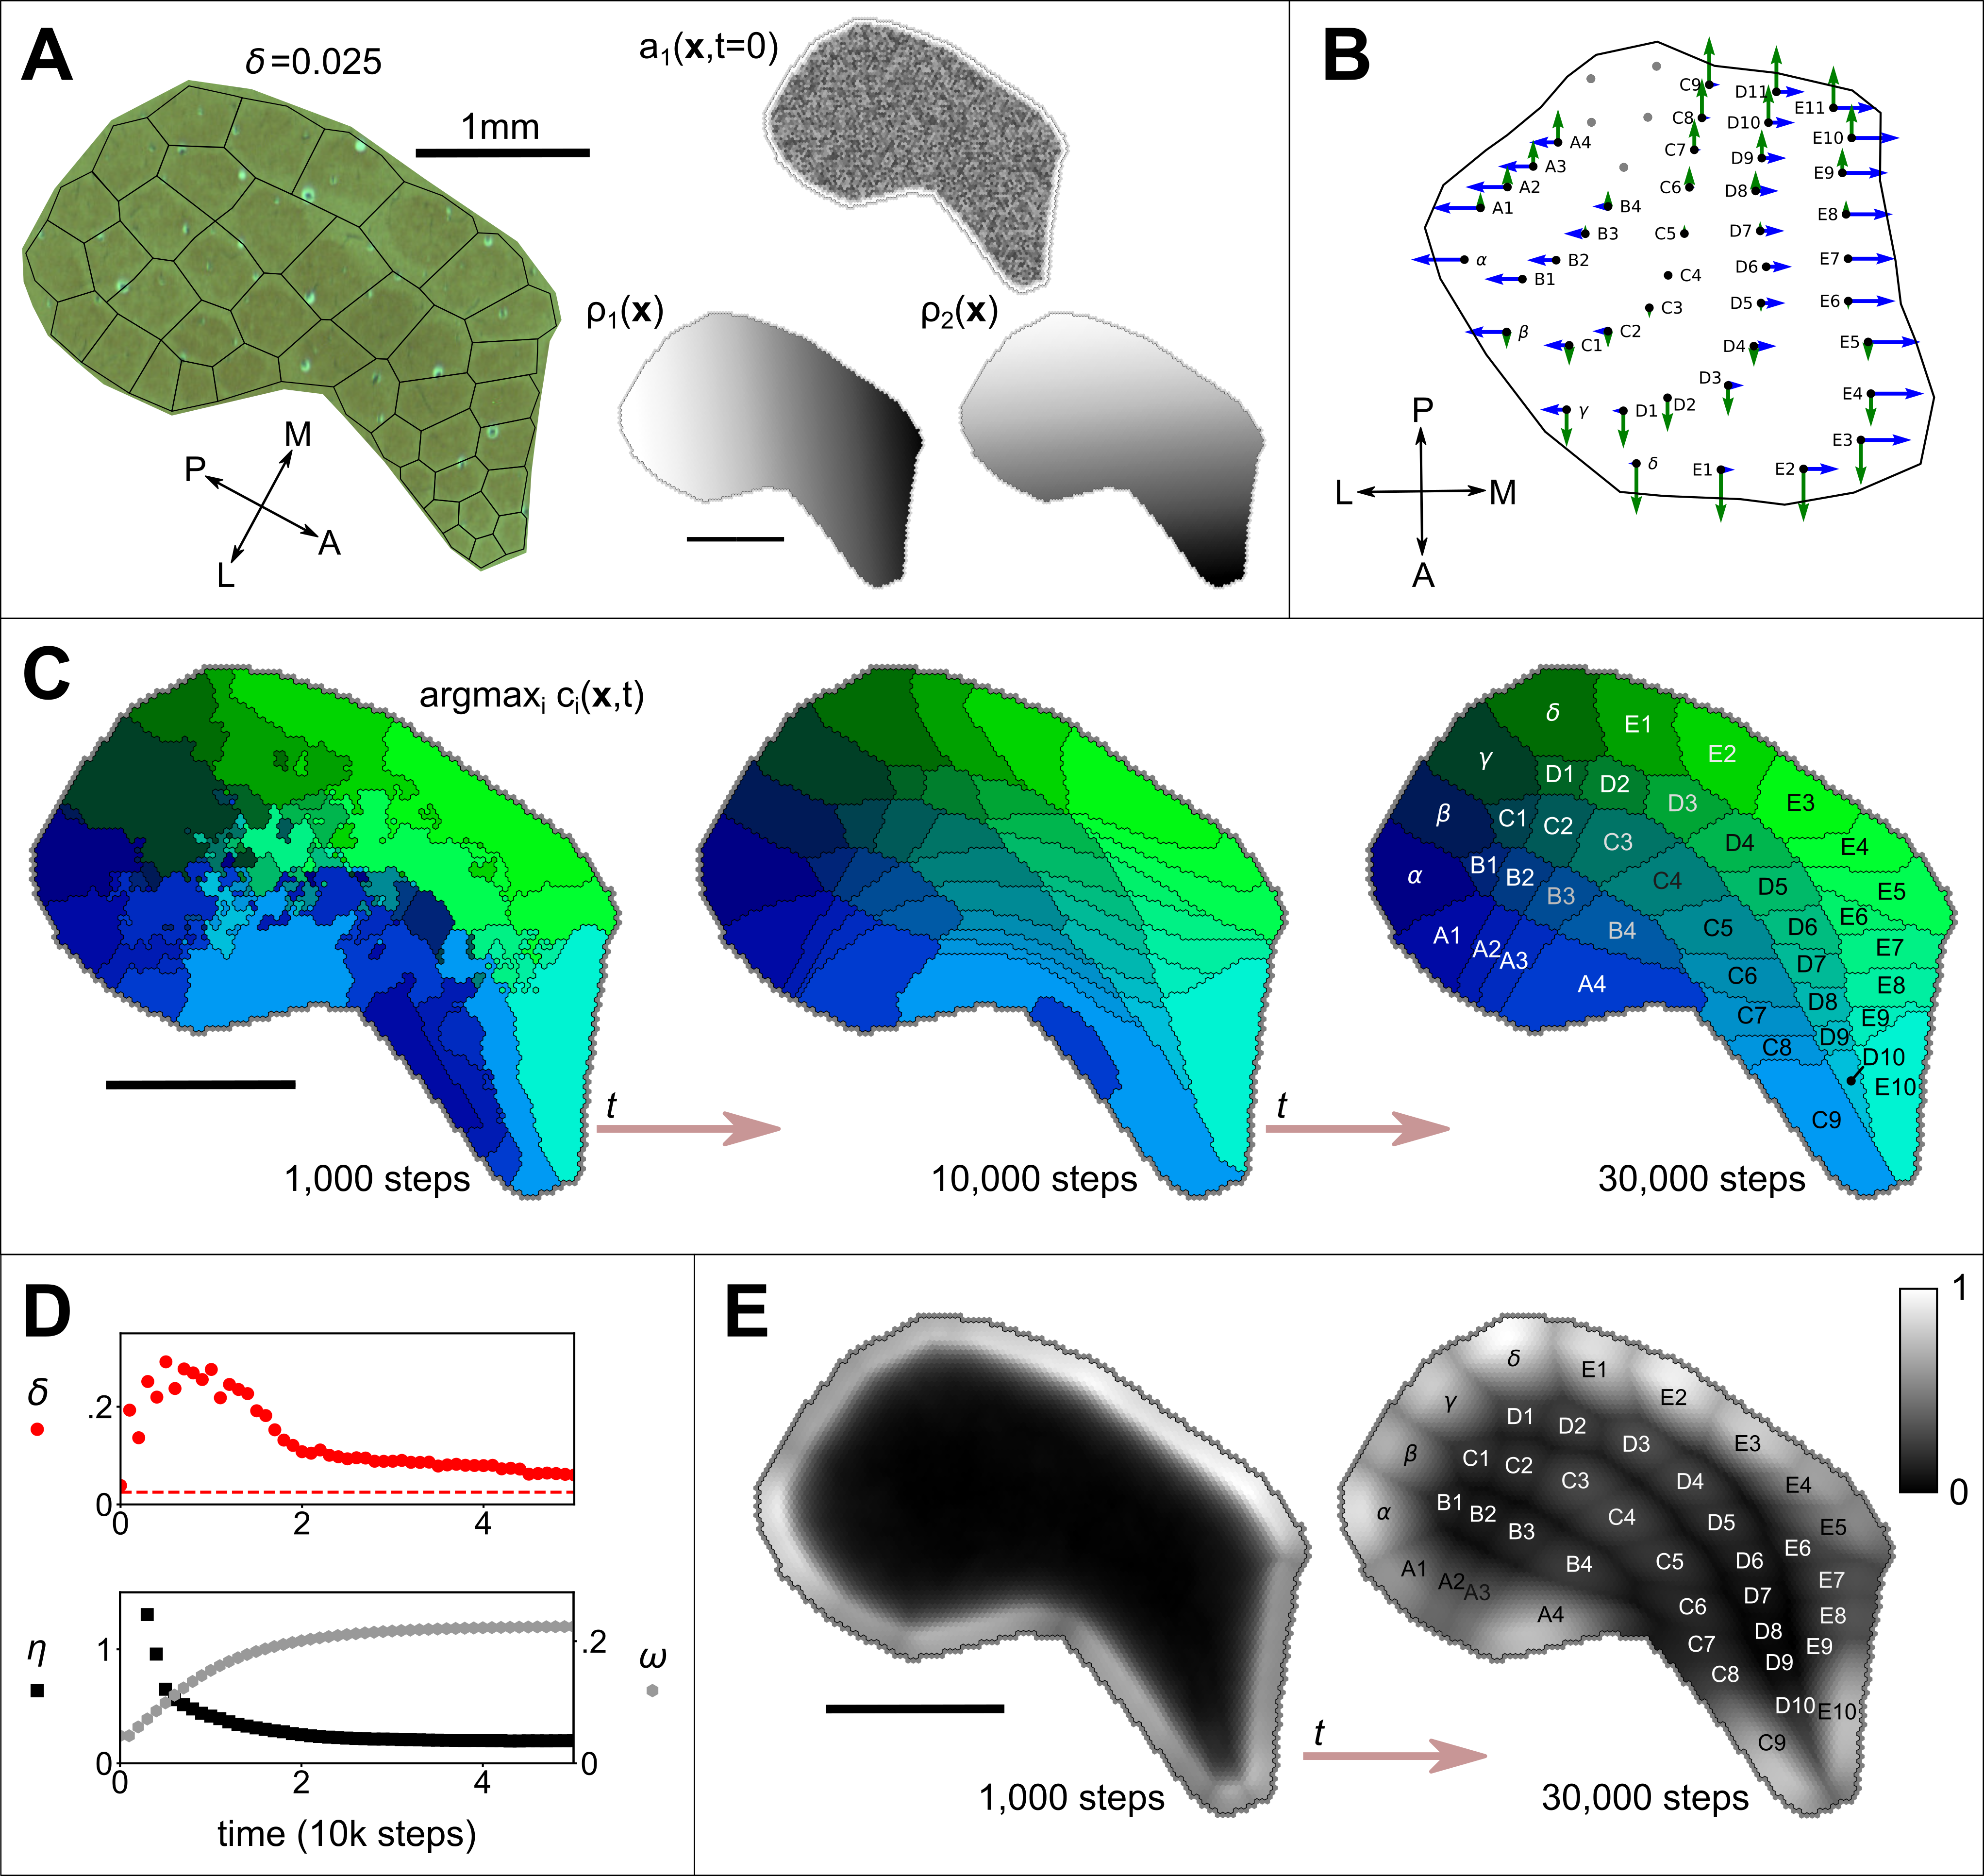
\includegraphics[width=\linewidth]{./Fig1.png}
    \caption{The emergence of whisker barrels.
      %
      \textbf{A} Left shows a cytochrome oxidase stain obtained from rat S1
      by \cite{zheng_signal_2001}, with black lines to delineate barrels and to
      measure departure (Honda-$\delta$; see \citealp{senft_mouse_1991}) from a
      perfect Voronoi tesselation. Right shows the initial distribution of axon
      branching density ($a$) for one thalamocortical projection, and two
      molecular guidance fields ($\rho$), \cmnt{where the domain $S$ has been
        traced from \textbf{A}}.
      %
      \textbf{B} The strengths of interaction $\gamma$ with fields $\rho_1$
      and $\rho_2$ are indicated for each of 41 projections by the lengths of
      green and blue arrows respectively, assuming that similar fields aligned
      to the posterior-anterior and medial-lateral axes in the ventroposterior
      medial nucleus of the thalamus are sampled at the locations of putative
      barreloid centers (reconstructed from \citealp{haidarliu_size_2001},
      their \cmnt{Fig.\,5b}).
      %
      \textbf{C} Results for the example simulation, with parameters
      \cmnt{$N=41$, $\alpha=3.6$, $\beta=16.67$, $k=3$, $D=0.5$,
        $\gamma\in\pm 2$, $\epsilon=1.2$} and $\delta{t}=0.0001$. Colours
      indicate the thalamic projection for which the connection density is
      maximal, \cmnt{barrel labels are located at the centroid of each
        region and} black lines delineate boundaries (see Movie S1).
      %
      \textbf{D} Red dots show the \emph{Honda}--\cmnt{$\delta(t)$} metric
      obtained from \cmnt{the} simulation approaching that obtained from
      the \cmnt{real} barrels in \textbf{A} (dotted line); black squares
      show the \emph{pattern difference} metric $\eta(t)$, and reveal the
      emergence of a correspondence between the real and simulated barrel
      shapes (units mm$^3$); \cmnt{grey hexagons show how selectively each
        cortical site is innervated;
        $\omega(t) = \oiint_{S} \mu(\mb{x},t) \mathrm{d}S$, where
        $\mu(\mb{x}) \equiv \mathrm{max}_i\big(c_i(\mb{x},t)\big)\big/\sum_{j=1}^{N} c_j(\mb{x},t)$.}
      %
      \textbf{E} \cmnt{Plotted across the cortical sheet, the selectivity
        develops to reveal an alignment with the emergent barrel boundary
        shapes}. \cmnt{Greyscale colour indicates values of $\mu(\mb{x})$.}
      All scale bars 1\,mm.}
    \label{fig:main}
  \end{fullwidth}
\end{figure}

First we verified that all results established by \cite{karbowski_model_2004}
for a 1D axis could be reproduced using our extension to a 2D cortical
sheet. Using an elliptical domain, $S$, with $M=3$ offset guidance gradients
aligned to the longer axis, $N=5$ thalamocortical projections gave rise to
five distinct cortical fields at locations that preserved the topographic
ordering defined by the original $\gamma$ values. However, we found that
specifying $N$ ordered areas required $M\approx (N+1)/2$ signalling
fields. This is because localization of axon densities occurs only when
projections are influenced by interactions with two or more signalling
gradients that encourage migration in opposing directions. As the number of
guidance fields is unlikely to approach the number of individual barrels,
\cmnt{modifications to the model} were required.

\cmnt{We reasoned that an arbitrary number of distinct field locations may
  be determined by a minimum of two guidance gradients, if the concentration
  of the projection densities is influenced by competition between
  projections, and if a projection that interacts more strongly with a given
  guidance gradient migrates further in the direction of that gradient.
  Accordingly, projections that interact most strongly with a given
  guidance gradient would come to occupy cortical locations at which that
  field has extreme values, leaving adjacent locations available to be
  occupied by projections with the next strongest interactions, and so
  forth. This would in principle allow the \emph{relative} locations of the
  fields to be specified by the relative values of the interaction parameters,
  $\gamma$, and hence for a topological map in the cortex to be specified by a
  spatial ordering of the $\gamma$ values at the level of the thalamus.}

\cmnt{Such dynamics are quite unlike those described by classic
  chemospecificity models} \citep{sperry_chemoaffinity_1963}, \cmnt{which
  essentially assume center-points by specifying conditions in the target
  tissue that instruct pre-identified afferents to stop growing. Consider, for
  example, that when simulated in isolation from one-another, all projections
  in the model described would simply migrate to the extrema of the cortical
  guidance fields.}

\cmnt{Testing this reasoning required increasing the strength of the
  competition between simulated thalamocortical projections for cortical
  territory, by increasing the tendency for each projection to compete for
  cortical space in which to branch and make connections. The major
  modification required
  was thus to introduce into the model an additional source of competition
  between thalamic projections.}
%
The term in parentheses in Eq.\,\ref{eq:dc} represents competition between
thalamocortical projections for a limited availability of cortical
connections. To introduce competition also in terms of axon branching,
\cmnt{whilst ensuring that $a_i$ is conserved over time,} we
redefined
%
\begin{equation} \label{eq:comp}
  \color{colcmnt}
  \chi_i(\mb{x}, t) = \frac{\epsilon a_i}{N-1} \nabla \textstyle\sum_{j\ne i}^{N}{a_j}.
  \color{black}
\end{equation}
%
\cmnt{This term contributes to the \emph{flux} of axonal branching as an
  additional source of diffusion, scaled by $\epsilon$, which reduces the
  branching density for a given projection where the branches of other
  projections are dense. Note that this operation is local to individual
  afferent projections.}

\cmnt{In addition, the model we have outlined requires that molecular
  guidance gradients in the cortex are complemented by graded values of the
  interaction strengths, $\gamma$, at the level of the thalamus. While the
  precise mechanisms by which thalamic and cortical gradients interact during
  development have not been fully characterised, the presence of complementary
  thalamic and cortical guidance gradients has been well established
  experimentally. In particular, the EphA4 receptor and its ligand ephrin-A5
  are distributed in complementary gradients in the somatosensory thalamus and
  cortex} (\citealp{vanderhaeghen_mapping_2000,miller_epha7-ephrin-a5_2006}).

\cmnt{Cells originating in VPM express high levels of EphA receptors and
  project to the lateral part of S1, which expresses low levels of ephrin-A5,
  and cells originating in the VPL express low levels of EphA receptors and
  project to the medial part of S1, which expresses high levels of ephrin-A5}
(see
\citealp{gao_regulation_1998,dufour_area_2003,vanderhaeghen_developmental_2004,speer_grading_2005,torii_role_2013}).
\cmnt{We assume that such patterning arises because the relative strengths of
  interaction with guidance molecules (e.g., ephrin-A5) in the cortex are
  correlated with the relative concentrations of complementary molecules
  (e.g., EphA4) in the thalamus, and thus with thalamic position along the
  axis to which their gradients are aligned.}

\cmnt{For simplicity, the two simulated thalamic interaction gradients, as
  well as the two cortical guidance gradients, were initially chosen to be
  linear and orthogonal. Hence a given pair of $\gamma$ values corresponds to
  the coordinate of a barreloid center in the VPM. Coordinates, in a reference
  plane defined by the anterior-posterior and medial-lateral axes, were
  estimated from Fig 5d of} \cite{haidarliu_size_2001}, \cmnt{and scaled
  such that $\gamma\in\pm 2$. Note that this scaling is arbitrary because
  according to the model the coordinates provide relative position information
  only.}

A cortical boundary enclosing barrels for 41 \cmnt{macrovibrissae} was
traced from a cytochrome oxidase stain from \cite{zheng_signal_2001}
\cmnt{(using original data kindly supplied by the authors)}, and
Eqs.~\ref{eq:dc}--\ref{eq:comp} were solved for $N=41$ projections on the
resulting domain, $S$, using $M=2$ linear signalling gradients aligned with
the anterior-posterior and medial-lateral axes.  \cmnt{These gradients are
  shown with the barrel field boundary in Fig.\,\ref{fig:main}A for clarity,
  though like ephrin-5 they may be thought of as extending across the cortical
  hemisphere \citep{miller_epha7-ephrin-a5_2006}. Simulations were stepped
  through 30000 iterations of Eqs.\,\ref{eq:dc}--\ref{eq:comp} ($\delta
  t=0.0001$).}

\cmnt{Across a wide range of parameter values, random initial conditions (a
  uniform random distribution for $a(\mb{x},0)\in(0.2,0.4)$, $c(\mb{x},0)=0$)
  eventually yielded a clear Voronoi-like tessellation of topographically
  organized thalamocortical projections, confirming that barrel maps can
  self-organize in the absence of pre-specified center points. The
  organization is apparent in a plot of the identity of the projection for
  which the connection density is maximal at each simulated cortical location,
  as shown in Fig.\,\ref{fig:main}C. Parameter values for this example simulation
  (see also Movie S1) were obtained by
  conducting a full parameter sweep and choosing a combination
  ($\alpha=3.6$, $\beta=16.67$, $k=3$, $D=0.5$, $\epsilon=1.2$) that scored
  well against the following three measures.}

% New section to describe and introduce the metrics
\cmnt{First, we used an algorithm introduced by Honda to measure the
  discrepancy of each barrel shape from a Dirichletform shape}
\citep{honda_geometrical_1983}.  \cmnt{Low overall values of this
  \emph{Honda-}$\delta$ metric obtained from simulated barrels indicate a
  close correspondence of the simulated barrel field with a Voronoi
  tesselation, and thus with a biological barrel field
  (for mice $\delta\approx0.054$,} \citealp{senft_mouse_1991}\cmnt{, and
  our analysis of data from} \citealp{zheng_signal_2001} \cmnt{ indicates that
  the value for rats is similar). For the tesselation
  that is overlaid on the real barrel field in Fig.\,\ref{fig:main}A,
  $\delta=0.025$, and a reduction in $\delta$ in the example simulation over
  time confirmed that an equivalent `good' Voronoi pattern can emerge
  within $\approx$~20000
  iterations (Fig.\,\ref{fig:main}D, red circles). Second, we devised a
  \emph{pattern difference} measure that is sensitive to deviations in the
  component shapes and overall topographic registration between two
  tesselations, $\eta$, and we used this measure to compare the simulated
  barrel fields to the real barrel field from which the boundary shape applied
  to the simulation was obtained (see \emph{Materials \& Methods} for
  details). A similar reduction in $\eta$ in the development of the example
  simulation confirmed that the shapes and arrangement of emergent connection
  fields came to match those of the real barrel field by around 20000
  iterations (Fig.\,\ref{fig:main}D, black squares). Third, we measured the
  \emph{connection selectivity} at each location on the cortical sheet, as the
  connection density of the most dense projection divided by the sum over all
  projection densities, $\omega$. The overall connection selectivity increased as the
  barrel map self-organized in the example simulation (Fig.\,\ref{fig:main}D,
  grey hexagons), and the selectivity became concentrated in regions
  overlapping with the emergent barrel centers (Fig.\,\ref{fig:main}E).}

% Full page width
\begin{figure}
  \begin{fullwidth}
    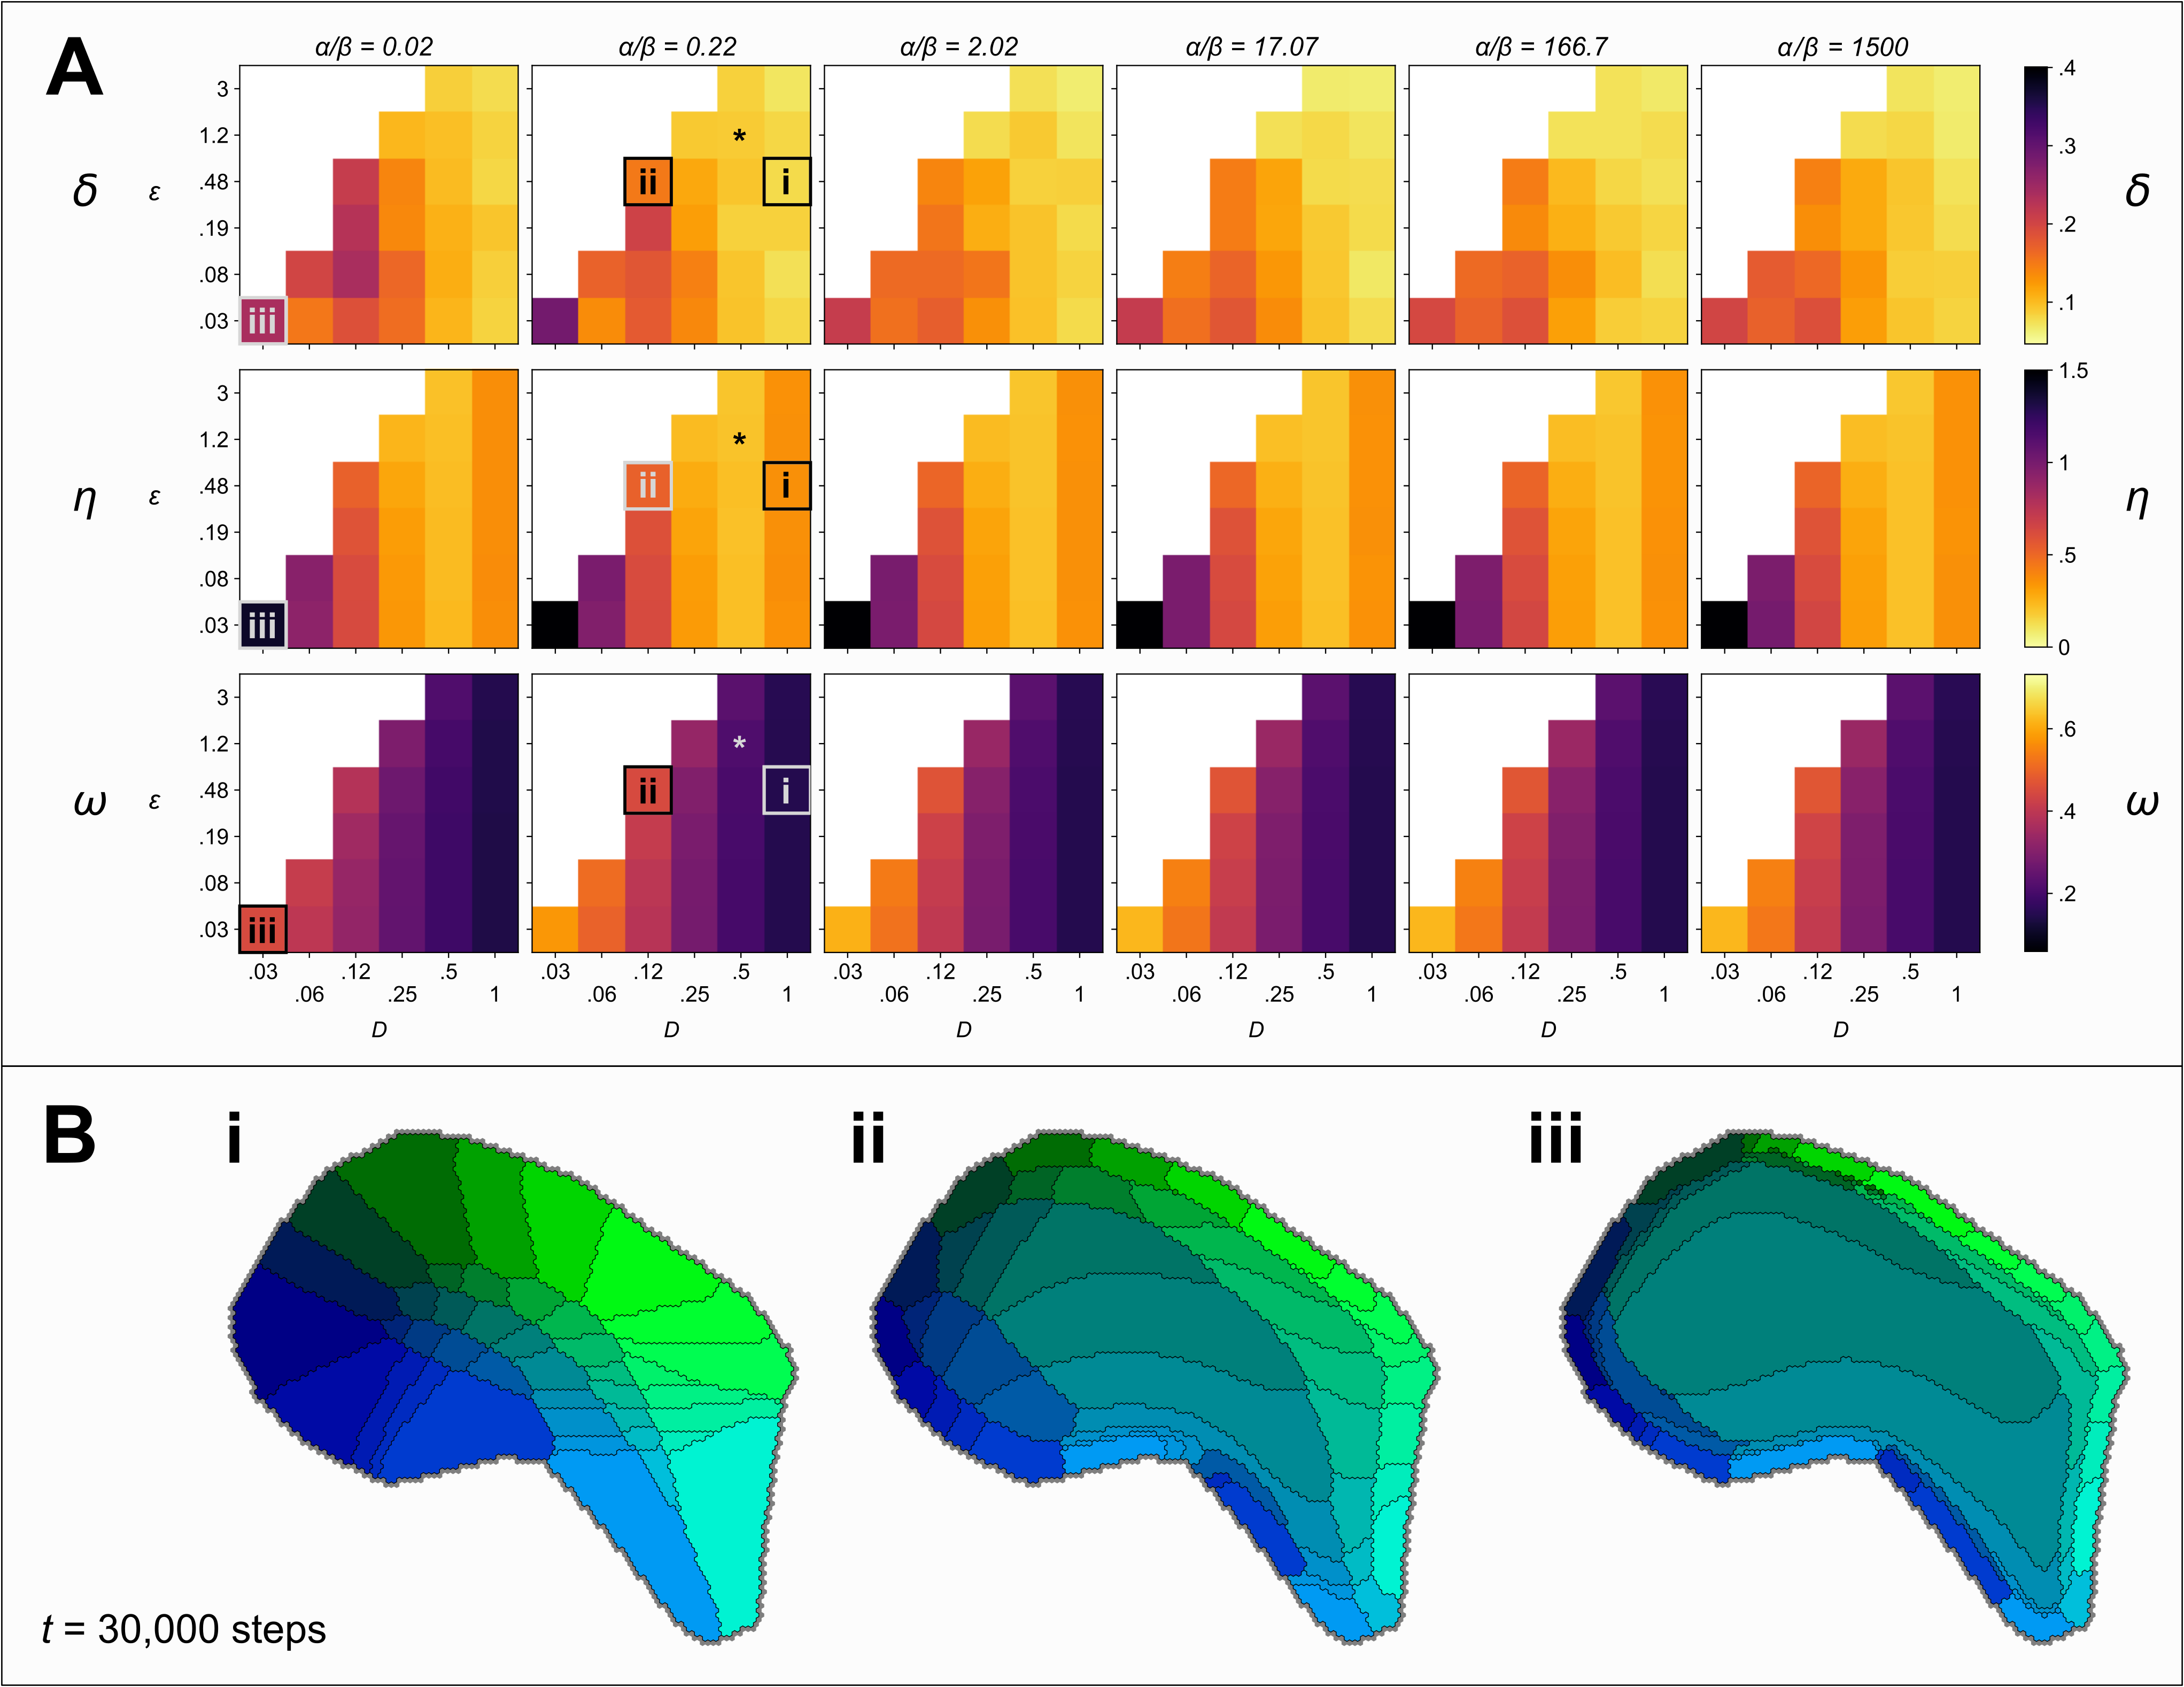
\includegraphics[width=\linewidth]{./Fig2.png}
    \caption{\cmnt{Exploring the parameter space.
        %
        \textbf{A} Colour indicates the quality of the pattern at $t=30000$
        steps, against three measures: Low values of \emph{Honda}--$\delta$
        (top row) suggest a Voronoi-like pattern of fields. The \emph{pattern
          difference}, $\eta$ (middle row) measures the difference in the area
        and arrangement of barrels in real and simulated fields. The
        \emph{selectivity}, $\omega$ (bottom row), measures the specificity
        with which the cortical sheet is innervated. Colour maps are chosen so
        that lighter (orange and yellow) colours indicate higher quality
        patterns against each measure. White squares indicate combinations of
        parameters for which simulations were numerically unstable.
        %
        The parameter space explored is three dimensional with the ratio
        $\alpha/\beta$ varying between plots, and the competition parameter
        $\epsilon$ and the diffusion constant $D$ varying within plots. An
        asterisk (*) marks the parameters used in Fig.\,\ref{fig:main}. Boxes
        i), ii)~and iii)~mark parameter sets for which corresponding patterns
        are shown in \textbf{B} (for $t=30000$ steps).
        %
        \textbf{B} Varying the diffusion constant $D$ generates qualitatively
        different patterns. Higher values cause expansions of the peripheral
        barrels and a corresponding compression of the inner barrels
        (i). Lower values instead cause an expansion of the central barrels
        and compression of the peripheral barrels (ii). Further reducing the
        rate of diffusion (iii), which is equivalent to increasing the size of
        the domain and hence simulating development in an animal with a larger
        cortex, causes a large area to be occupied by projections with
        intermediate interaction parameters; those with strong interaction
        parameters are compressed around the edge of the domain, and
        consequently a barrel pattern fails to form.}}
    \label{fig:paramsweep}
  \end{fullwidth}
\end{figure}

\cmnt{Against these three metrics we are also able to characterise the
  robustness of self-organization to the model parameters, and to investigate
  the sensitivity of the model to variation in its inputs.} \cmnt{Fig.\,\ref{fig:paramsweep}A shows values of $\delta$, $\eta$ and
  $\omega$ obtained after 30000 iterations, from 216 independent simulations,
  each representing a unique combination of the model parameters $D$,
  $\epsilon$, and the ratio $\alpha/\beta$. First we observe that
  self-organization is highly robust to the ratio $\alpha/\beta$, across five
  orders of magnitude, with respect to all three metrics. Second, the most
  strongly Dirichletform patterns (low \emph{Honda}-$\delta$) were generated
  by simulations in which the diffusion constant $D$ and the strength of
  competition $\epsilon$ were high. Third, strongest overall connection selectivities,
  $\omega$, were obtained for lower values of $D$. Fourth, variation in the
  pattern difference metric, $\eta$, indicated that the alignment between real
  and simulated patterns was greatest for intermediate rates of diffusion,
  $D\approx0.5$. Together these results indicate that when competition is
  strong, the rate of diffusion determines a trade-off such that fields emerge
  to be barrel-shaped when diffusion is fast and they emerge to be more
  selectively innervated when diffusion is slow.}

\cmnt{The parameters of the example simulation are indicated in
  Fig.\,\ref{fig:paramsweep}A using an asterisk. In
  Fig.\,\ref{fig:paramsweep}B, we also present examples of alternative
  patterns that emerge for different choices of $D$. Decreasing the rate of
  diffusion may be considered equivalent to increasing the overall size of the
  domain, $S$. Hence, insights into barrel development in species with a
  larger representation of the vibrissae, which do not have barrel fields, may
  be gained by studying pattern formation
  when $D$ is small. In this context, it is interesting to note that for small
  $D$, the organization is predicted to be topological but highly irregular,
  with a general expansion in the territory occupied by the central versus
  peripheral domains that would presumably manifest as an absence of
  identifiable barrel fields (Fig.\,\ref{fig:paramsweep}B\,iii).}

% Full page width
\begin{figure}
  \begin{fullwidth}
    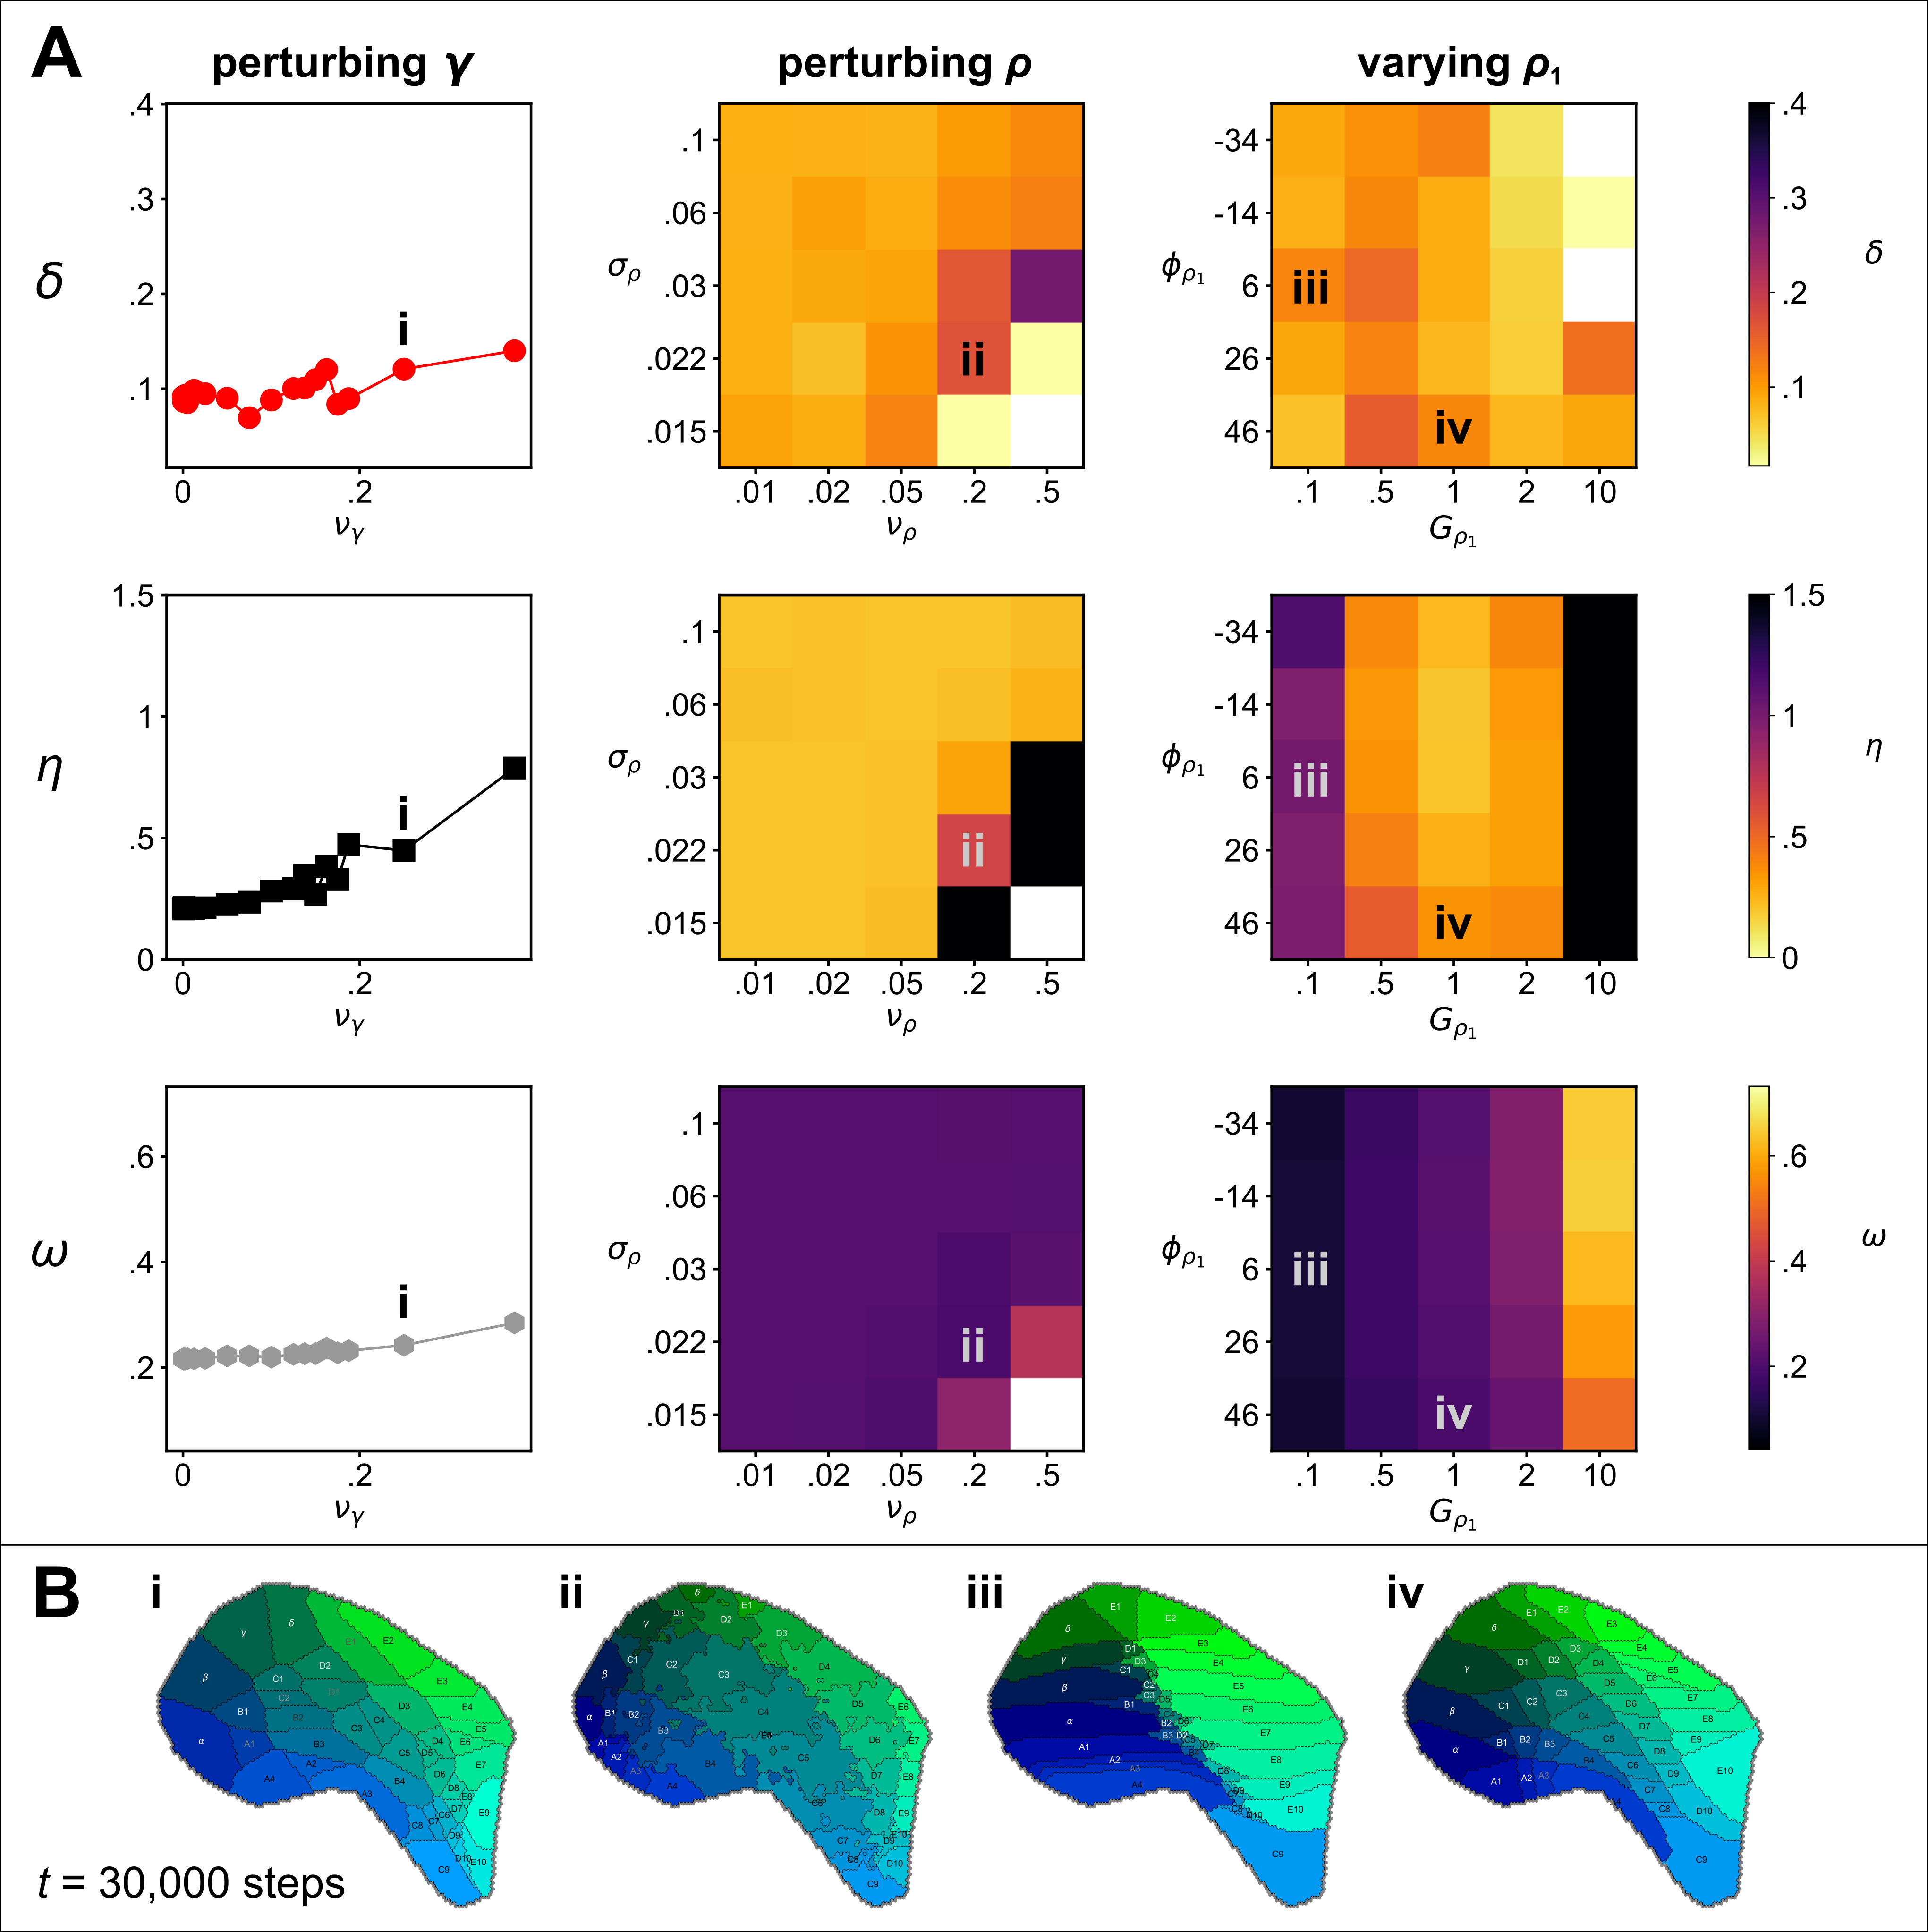
\includegraphics[width=\linewidth]{./Fig3.png}
    \caption{
      \cmnt{Sensitivity analysis.
        %
        \textbf{A} Metrics of map quality $\delta(t)$ (top row), $\omega(t)$
        (middle row) and $\eta(t)$ (bottom row), were evaluated at $t=30000$
        steps. The $y$-axes and colour scales have identical ranges to the
        colour scales in Fig.\,\ref{fig:paramsweep}, for easy comparison.
        %
        \emph{Left column:} The effect of adding noise drawn from a uniform
        distribution, $(\gamma_{max}-\gamma_{min})\,U(0,\nu_\gamma)$, to the
        values of the interaction parameters, $\gamma$ used in
        Fig.\,\ref{fig:main}.
        %
        \emph{Middle column:} The effect of changing the magnitude and the
        length scale of noise applied to the guidance fields. Uniform random
        noise $(\rho_{max} - \rho_{min})\,U(0, \nu_{\rho})$ was added to each
        (hexagonal) element of $\rho_1(\mb{x})$ and $\rho_2(\mb{x})$ and the
        result was smoothed by convolution with a symmetric 2D Gaussian kernel
        of width $\sigma_\rho$.
        %
        \emph{Right column:} The effect of setting the rotational angle of the
        linearly varying guidance field, $\rho_1(\mb{x})$, to $\phi_{\rho_1}$,
        and modifying its overall gain to $G_{\rho_1}$, whilst keeping the
        parameters of $\rho_2(\mb{x})$ unchanged from those used in the
        example simulation, for which $\phi_{\rho_2}=84$\textdegree and
        $G_{\rho_2}=1$.
        %
        \textbf{B} Four ways in which the perturbations in \textbf{A} affect
        the patterns. i) The effect of significant interaction parameter noise
        results in topological defects. ii) High magnitude, short lengthscale
        noise in $\rho(\mb{x})$ leads to non-straight edges between adjacent
        barrels. iii) Reducing the slope of gradient $\rho_1$ (by a factor of
        10) causes barrel rows B, C and D to become `crushed' down the center
        line, and edge barrels to dominate. iv) Rotating $\rho_1$ by
        20\textdegree~causes a slight distortion of the pattern, resulting in
        an overall anticlockwise rotation of the field locations. }}
    \label{fig:sens}
  \end{fullwidth}
\end{figure}


\cmnt{Next we conducted a sensitivity analysis to determine the extent
  to which the quality of the pattern (after $t=30000$ iterations) is affected
  by perturbations to i)~the magnitude and offset of the noise applied to
  $a_i$ at $t=0$; ii)~noise applied to the interaction parameters,
  $\gamma_{i,j}$; iii)~noise (at various length scales) applied to the
  guidance fields; and iv)~the magnitude and orientation of one cortical
  guidance field relative to the other (Fig.\,\ref{fig:main}A).}

\cmnt{Using the parameters of the example simulation
  (Fig.\,\ref{fig:main}C) we established baseline mean and standard deviations
  from ten independent simulations with initial uniform random values for
  $a(\mb{x},0)\in(0.2,0.4)$, to be $\delta=0.089\pm 0.004$, $\eta=0.2108\pm
  0.002$, and $\omega=0.2165\pm 0.0001$. Repeating with the variation in the
  initial noise doubled ($a(\mb{x},0)\in(0.1,0.5)$), or removed altogether
  ($a(\mb{x},0)=0.3$), generated distributions of $\delta$, $\eta$, and
  $\omega$ that were not statistically different, as established using paired
  two-sample t-tests. Adding noise to the interaction parameters ($\gamma$)
  affected neither the \emph{Honda-}$\delta$ or the \emph{connection
    selectivity} measures substantially (see Fig.\,\ref{fig:sens}A), and an
  increase in the \emph{pattern difference} reflected an increase in the
  occurrence of topological defects only when perturbations become so large as
  to cause the ordering of $\gamma$ values from neighbouring thalamic sites to
  be switched (see example map Fig.\,\ref{fig:sens}B\,i). Adding noise to the
  cortical guidance field values, $\rho_1(\mathbf{x})$ and
  $\rho_2(\mathbf{x})$, disrupted pattern formation only for high levels of
  noise applied at short length scales, which manifested as non-straight edges
  at the domain boundaries (Fig.\,\ref{fig:sens}B\,ii). Varying the slope of one
  linear gradient $\rho_1(\mathbf{x})$ while keeping that of the other
  constant caused elongation of the emergent domains along the corresponding
  axis (Fig.\,\ref{fig:sens}B\,iii), while pattern formation was not strongly
  influenced by relaxing the assumption that the gradients of the two cortical
  guidance fields are orthogonal (Fig.\,\ref{fig:sens}B\,iv). Overall, the
  sensitivity analysis revealed that self-organization of barrel-like fields
  in the model is highly robust to a wide range of sources of perturbation.}

\cmnt{To further investigate the interplay of genes intrinsic to the
  developing neocortex and extrinsic factors such as thalamocortical input,
  we simulated two well known experimental manipulations of barrel
  development. First, we simulated a seminal barrel duplication paradigm}
\citep{shimogori_fibroblast_2005,assimacopoulos_fibroblast_2012}
\cmnt{in which the growth factor Fgf8, which is normally expressed at
  the anterior end of the cortical subplate from around E9.5}
\citep{crossley_mouse_1995}, \cmnt{is ectopically expressed (by
  electroporation) also at the posterior pole. We assume that this results in
  a mirror of the primary barrel cortex boundary along the rostrocaudal axis}
\citep{assimacopoulos_fibroblast_2012} \cmnt{and a mirroring of the
  anterior-posterior guidance gradient $\rho_1$ at the border between them
  (Fig.\,\ref{fig:fgf8}A). The result after 30000 iterations, and otherwise
  using the parameters of the example simulation, was two mirror-symmetrical
  barrel fields comprising $2N$ barrels (Fig.\,\ref{fig:fgf8}B), consistent
  with the outcome of the original experiments.}

% This figure is text width
\begin{center}
  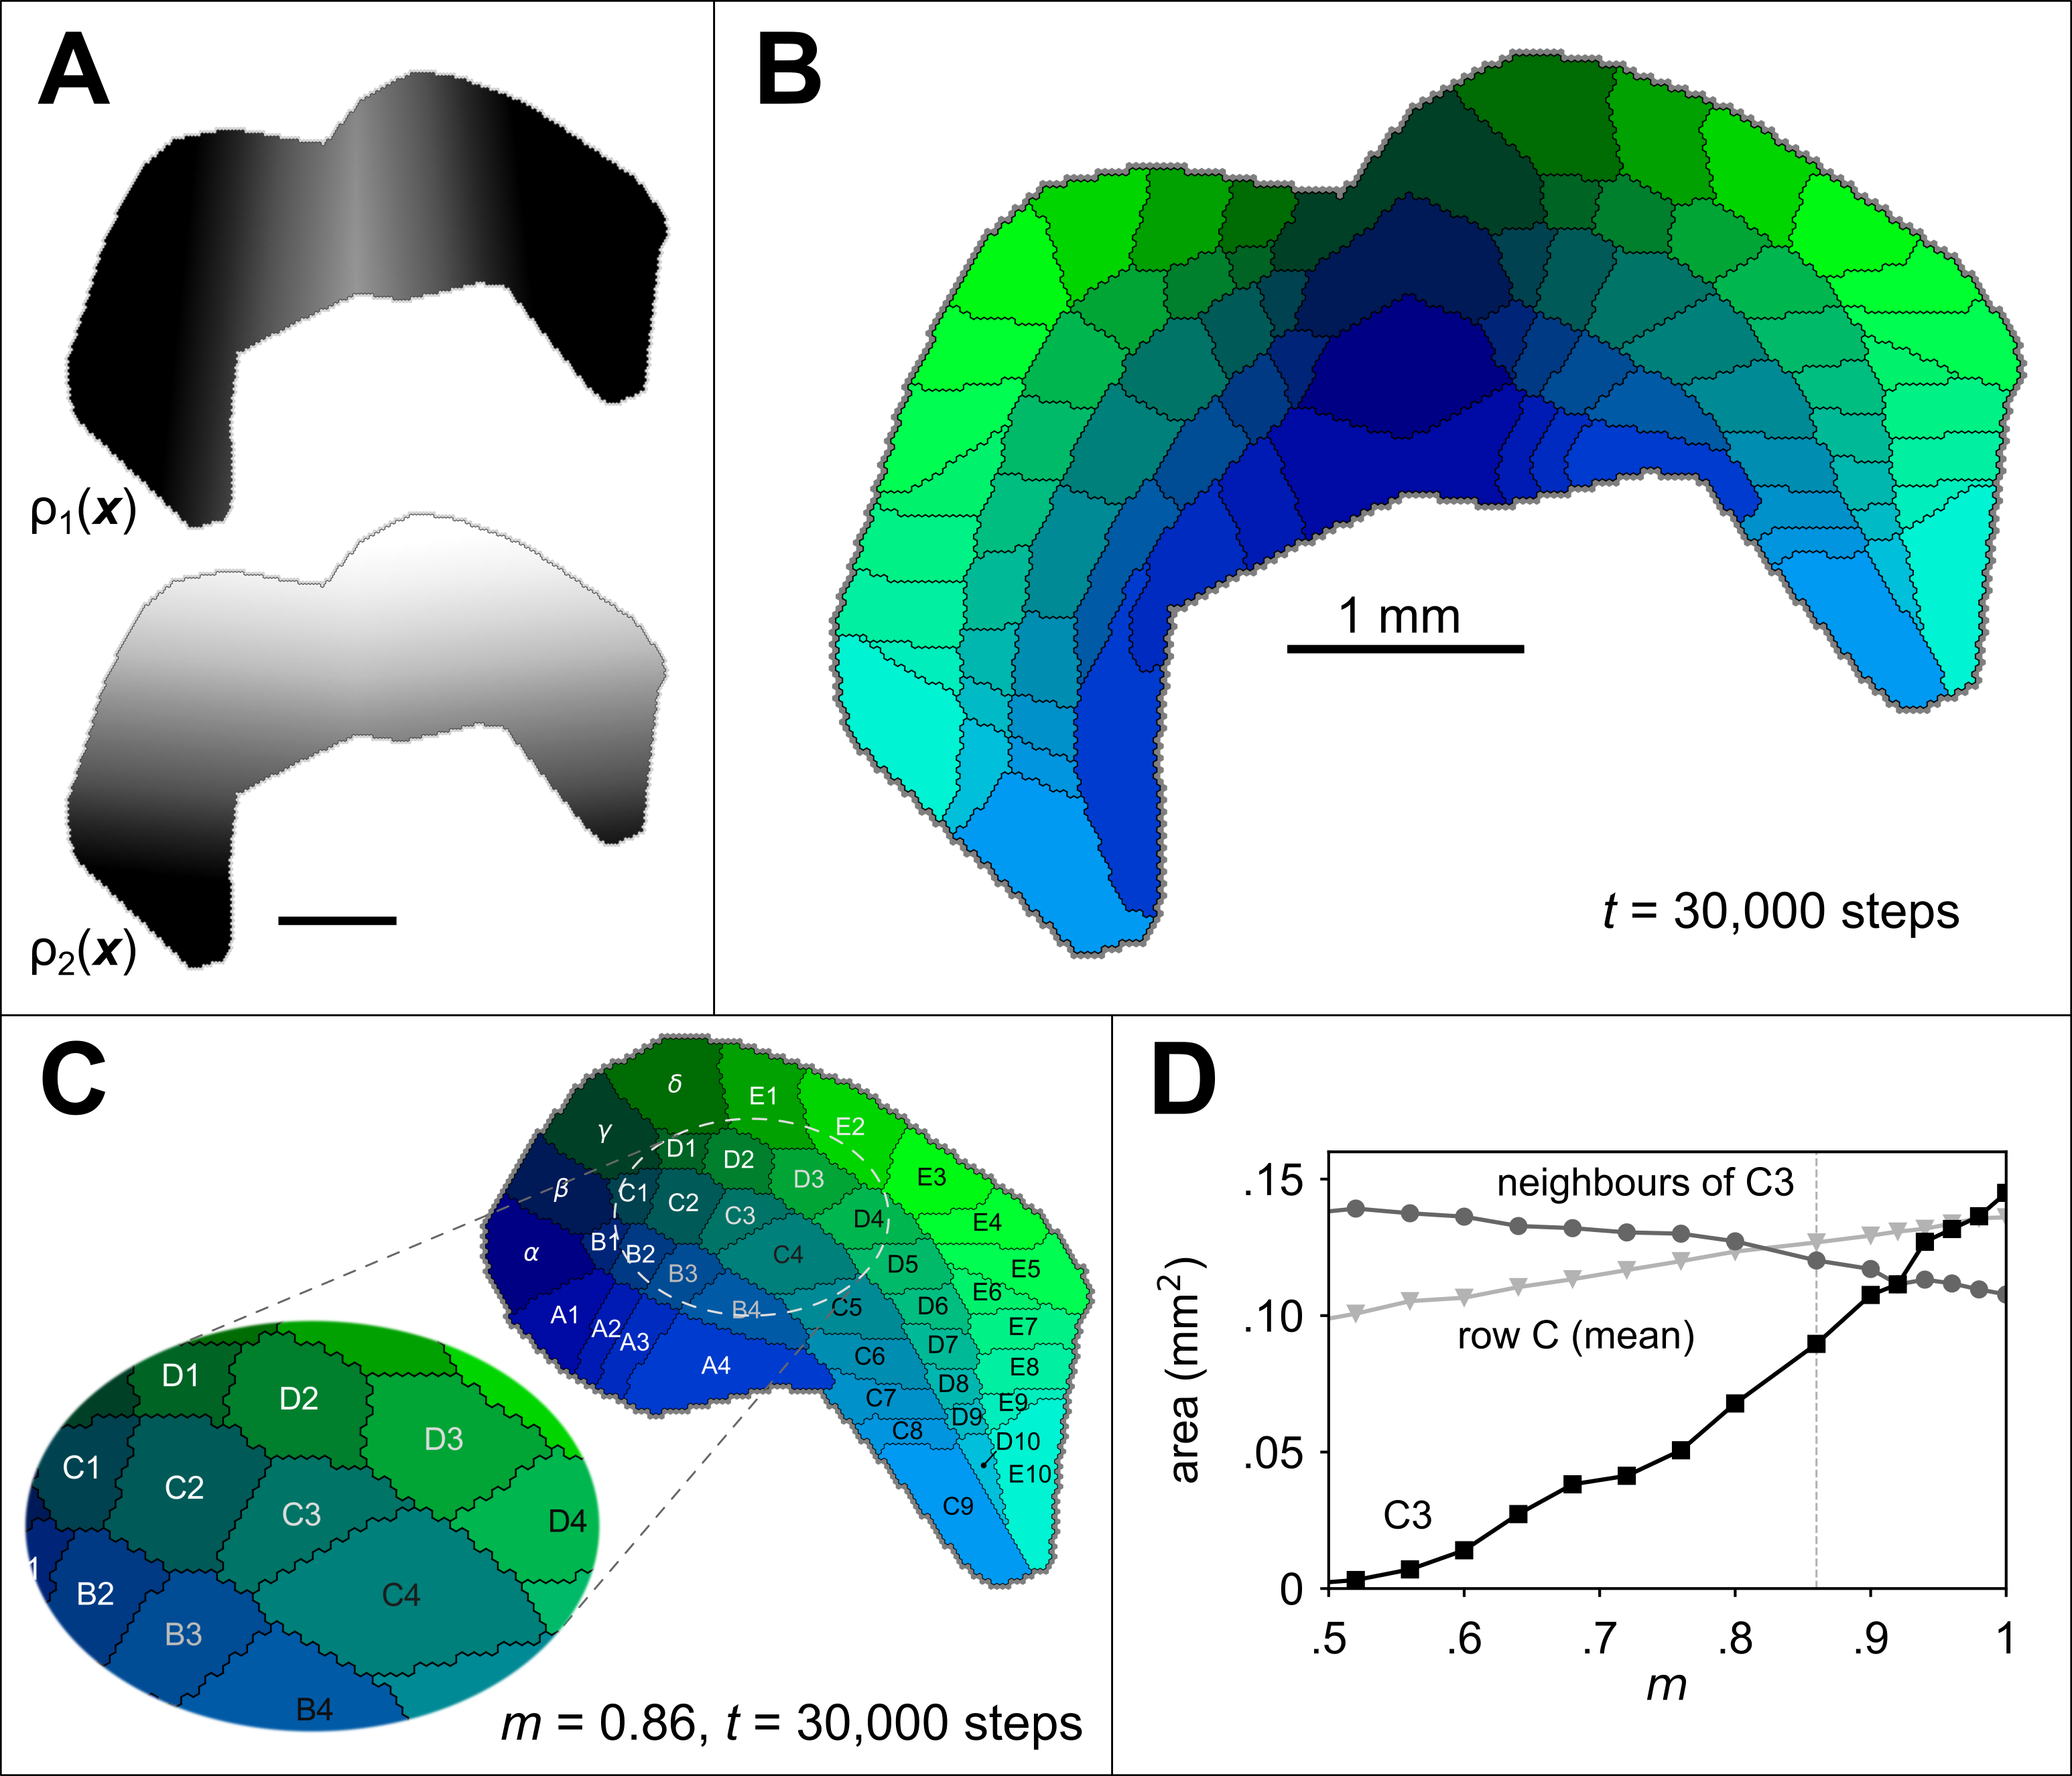
\includegraphics[width=\linewidth]{./Fig4.png} \captionof{figure}{
    \cmnt{Simulating altered barrel development.  Guidance fields
      (\textbf{A}) and emergent barrel pattern (\textbf{B}) in a Fgf8
      misexpression experiment
      (c.f.~\citealp{assimacopoulos_fibroblast_2012}), simulated by reflecting
      $\rho_1$ from Fig.\,\ref{fig:main}A at the join of the original boundary
      with its mirror. All other model parameters match those in
      Fig.\,\ref{fig:main}C. \textbf{C} Simulating whisker trimming by
      reducing the competitiveness, $\epsilon$, of one projection. For C3
      only, $\epsilon$ was mutiplied by $m\in(0,1)$. The pattern shown is that
      formed after 30000 steps with $m=0.86$, which reduces the size of the C3
      field to 65\% of its original size, matching the average barrel area
      reduction observed by }
    \cite{kossut_effects_1992}. \cmnt{\textbf{D} The area of the C3
      barrel (black squares) reduces as $m$ is reduced, whereas the mean area
      of neighbouring barrels (B3, C2, C4, D2 \& D3, grey circles)
      increases. The dotted grey line indicates $m=0.86$ for comparison with
      panel \textbf{C}. If the $\epsilon$ value is instead reduced for \emph{all} row C
      projections (including the interstitial $\gamma$ projection), the mean
      row C barrel area is only slightly reduced (light grey triangles). In
      this case, the mean area of a simulated row C barrel at $m=0.86$ is 91\%
      of that for $m=1$.}}
  \label{fig:fgf8}
\end{center}

\cmnt{Finally, to investigate the response of the model to
  environmental manipulation, we simulated a whisker deprivation
  experiment. In a critical period comprising the first postnatal days,
  removal of the whiskers by electrocauterization, plucking, or trimming leads
  to observable changes in brain structures, including the barrel
  field~\citep{jeanmonod_mouse_1981}. Amongst other changes, deprivation of
  individual whiskers leads to smaller
  % loos_somatosensory_1973 for row cauterization
  barrels~\citep{kossut_effects_1992}. We simulated
  trimming of the individual whisker C3 during the critical period by reducing
  the competitiveness of the C3 thalamocortical projection, $\epsilon$. As a
  result, the corresponding field size was smaller (Fig.\,\ref{fig:fgf8}C),
  and the size of the fields representing the neighbours of C3 increased in
  size. A reduction in area to 65\%, comparable to that induced by
  \cite{kossut_effects_1992}, was obtained in simulation when $\epsilon$
  was reduced to 86\% (Fig.\,\ref{fig:fgf8}D), and the C3 barrel disappeared
  altogether when $\epsilon$ was less than half of its original value.}

\cmnt{Although individual whisker trimming reduces barrel size, if an
  entire row is trimmed, barrel sizes for the trimmed row are not obviously
  changed \citep{land_metabolic_1985}. We investigated with a simulation in
  which we varied $\epsilon$ for all of the row C projections.  Although the
  barrels which formed for row C did show some reduction in area
  (Fig.\,\ref{fig:fgf8}D), this reduction was small when compared with the
  individually trimmed C3 simulation. If the effect of trimming any whisker is
  to reduce its $\epsilon$ (the competitiveness of its projection) to 86\% of
  its original value, then the model predicts that the cortical barrels for
  the trimmed C row will retain 91\% of their area on average.}

\cmnt{Together with the results of simulated misexpression, the
  consistency of the simulated whisker trimming results with those of the
  original studies demonstrates how the model can be used to investigate the
  contribution of intrinsic and extrinsic factors to the development of
  cortical fields.}

\section{Discussion}

The present results suggest that the key requirements for the emergence of
realistic barrel patterning are i)~at each cortical location thalamocortical
projections compete for a limited number of available synaptic connections
(Eqs.~\ref{eq:dc}--\ref{eq:da}), ii)~at each location the branching rate of a
given projection is reduced by the density of other projections
(Eq.\,\ref{eq:comp}), and iii)~the branch density of each projection is
conserved over time.

The emergence of barrels in simulation required competition between thalamic
projections in terms of synaptic connectivity and also competition in terms of
cortical space, as represented by $\chi$, with an implicit requirement for a
self/other identifier amongst projections. This latter form of competition may
account for the absence of barrels in rodents with larger brains, such as
capybara, for which competition for space is presumably weaker
\citep{woolsey_comparative_1975}. Hence, irrespective of whether barrels are
necessary for adaptive whisker function, the emergence of somatotopically
ordered modular structures may be an inevitable consequence of local
competition for cortical territory driven by input from an array of discrete
sensory organs \citep{purves_iterated_1992}.

\cmnt{In reality, scores of smaller Dirichletform barrels representing the
  microvibrissae form alongside the E-row barrels, presumably via the same
  competitive processes. Enforcing here
  the same boundary condition as used to represent the true edges of the
  barrel field was necessary to ensure the stability of the simulation, though
  we acknowledge that this region of the boundary was enforced primarily to
  keep the number of simulated projections, and hence the overall
  computational complexity of the simulation, manageable (simulating an extra
  projection introduces 13030 new dynamical variables).}

It is important to emphasize that the formulation of the model is entirely
local, insofar as simulation requires no information to be communicated from a
given cortical grid cell to any but those immediately adjacent (via
diffusion). Hence the simulations demonstrate how a self-organizing system,
constrained by genetically specified guidance cues and by the shape of the
cortical field boundary, can faithfully reproduce an arrangement of cell
aggregates in one neural structure as a topographic map in another.

Moreover, the present results confirm that somatotopic map formation does not
require the pre-specification of center-points by as yet undetermined
additional developmental mechanisms.

\section{Materials \& Methods}

% Be sure to include/mention:
%
% The no-flux boundary conditions applied in the \cite{karbowski_model_2004}
% model are retained.
%
% Arbitrary boundary shapes were applied

\cmnt{We concentrated on the representation of the forty-one macrovibrissae
  that constitute a given barrel field, because their thalamic and cortical
  correlates are easily identifiable and consistently located, excluding the
  five rhinal whiskers as their cortical representation is isolated from the
  main barrel field. We excluded the representation of the microvibrissae to
  limit the overall complexity of the simulations.}

The cortical sheet was modelled as a two dimensional hexagonal lattice, which
simplifies the computation of the 2D Laplacian. Within a boundary traced
around the edge of a rat barrel field (Fig.\,\ref{fig:main}A) we set the
hex-to-hex distance $d$ to 0.03\,mm, which resulted in a lattice containing
6515 hexes for the simulations shown in Figs.\,\ref{fig:main}A,C \& D and
12739 hexes for the Fgf8 misexpression study shown in
Fig.\,\ref{fig:fgf8}. Each hex contained 82 time-dependent variables: 41
branching densities ($a_i$) and 41 connection densities ($c_i$).  The rate of
change of each of the time-dependent variables (Eqs.\,\ref{eq:dc} \&
\ref{eq:da}) was computed using a fourth-order Runge-Kutta method.

The most involved part of this computation is to find the divergence of the
flux of axonal branching, $\mb{J}_i(\mb{x},t)$, the term in parentheses in
Eq.\,\ref{eq:da}:
%
\begin{equation}
  \label{eq:divJ}
  \nabla\vcdot\mb{J}_i(\mb{x},t) = \nabla\vcdot\left(D \nabla
  a_i-a_i\sum_{j=1}^{M} \gamma_{i,j}\nabla \rho_j(\mb{x}) \color{colcmnt}+
  \frac{\epsilon a_i}{N-1} \nabla \hat{a}_i \color{black}\right),
\end{equation}
%
\cmnt{where $\hat{a}_i\equiv\sum_{j\ne i}^{N}a_j$.} Note that the sum of the
guidance gradients is time-independent and define $\mb{g}_i(\mb{x}) \equiv
\sum_{j=1}^{M} \gamma_{i,j} \nabla\rho_j(\mb{x})$.  Because the divergence
operator is distributive, Eq.\,\ref{eq:divJ} can be expanded using vector
calculus identities (dropping references to $\mb{x}$ and $t$ for clarity):
%
\begin{equation}
\nabla\vcdot\mb{J}_i = \nabla\vcdot\big(D \nabla a_i\big) -
\nabla\vcdot\big(a_i \mb{g}_i\big) \color{colcmnt} + \frac{\epsilon}{N-1}\nabla\vcdot\big({a}_i\nabla\hat{a}_i\big)\color{black}.
\end{equation}
%
Applying the vector calculus product rule identity yields
%
\begin{equation} \label{eq:divJExpanded}
%
\nabla\vcdot\mb{J}_i =
%
D \dvrg a_i % term1
-
a_i\nabla\vcdot\mb{g}_i % term2
-
\mb{g}_i\vcdot\nabla a_i % term3
\color{colcmnt}
+ \frac{\epsilon a_i}{N-1} \dvrg \hat{a}_i % term1_1
+ \frac{\epsilon}{N-1} \nabla \hat{a}_i\vcdot\nabla{a}_i% term1_2
\color{black}
,
\end{equation}
%
which has \cmnt{five} elements to compute: i)~$D \dvrg a_i$ (the Laplacian of
$a_i$); ii)~a time-independent modulator of $a_i$ (because
$\nabla\vcdot\mb{g}_i$ is a time-independent static field); iii)~the scalar
product of the static vector field $\mb{g}_i$ and the gradient of $a_i$;
\cmnt{iv)~the Laplacian of $\hat{a}_i$; and v)~a term involving the gradients
  of $a_i$ and $\hat{a}_i$}. Each of the divergences can be simplified by
means of Gauss's Theorem following \cite{lee_hexagonal_2014}.

(i) The computation of the mean value of the Laplacian across one hexagon of
area $\Omega = \frac{\sqrt{3}}{2}d^2$, located at position $\mb{p}_0$, with
neighbours at positions $\mb{p}_1$--$\mb{p}_6$ is
%
\begin{equation} \label{eq:lapl}
\begin{split}
\langle D \dvrg a_i(\mb{p}_0,t) \rangle  = \frac{D}{\Omega} \oiint_\Omega \dvrg a_i(\mb{x}, t) \dif\Omega & = \frac{D}{\Omega} \oint \frac{\partial a_i}{\partial \hat{\mb{n}}} \dif\gamma \\
& \approx \frac{D}{\Omega} \sum_{j=1}^6 \frac{\partial a_i(\mb{p}_j)}{\partial \hat{\mb{n}}} \bigg\rvert_{\mathrm{mid}} v \\
& = \frac{2D}{\sqrt{3} d^2} \sum_{j=1}^6 \frac{a_i(\mb{p}_j) - a_i(\mb{p}_0)}{d} \frac{d}{\sqrt{3}} \\
& = \frac{2D}{3 d^2} \sum_{j=1}^6 \big(a_i(\mb{p}_j) - a_i(\mb{p}_0)\big),
\end{split}
\end{equation}
%
where $v = d/\sqrt{3}$ is the length of each edge of the hexagon and
$\dif\gamma$ is an infinitesimally small distance along its perimeter.

\noindent
ii) The computation of the second term in Eq.\,\ref{eq:divJExpanded},
$\langle a_i(\mb{p}_0,t)\nabla\vcdot\mb{g}_i(\mb{p}_0)\rangle$, can be written
out similarly:

\begin{equation} \label{eq:divg}
\begin{split}
%
\frac{1}{\Omega} \oiint_\Omega a_i\nabla\vcdot\mb{g}_i\;\dif\Omega & = \frac{a_i(\mb{p}_0,t)}{\Omega}  \oint \mb{g}_i\vcdot \dif\hat{\mathbf{n}} \\
%
& \approx \frac{a_i(\mb{p}_0,t)}{\Omega} \sum_{j=1}^{6} \frac{\mb{g}_i(\mb{p}_j) + \mb{g}_i(\mb{p}_0)}{2}\vcdot \hat{\mb{n}}\;v \\
%
& = \frac{2 a_i(\mb{p}_0,t)v}{\sqrt{3}d^2} \sum_{j=1}^{6} \bigg[ \frac{g_i^x(\mb{p}_j) + g_i^x(\mb{p}_0)}{2} \vcdot  \hat{\mb{n}} + \frac{g_i^y(\mb{p}_j) + g_i^y(\mb{p}_0)}{2} \vcdot  \hat{\mb{n}} \bigg] \\
%
%%& = \frac{2 a_i(\mb{p}_0,t)d}{\sqrt{3}d^2\sqrt{3}} \bigg( \sum_{j=1}^{6} \frac{\mb{g}_j^x + \mb{g}_0^x}{2} \vcdot  \hat{\mb{n}} + \sum_{j=1}^{6} \frac{\mb{g}_j^y + \mb{g}_0^y}{2} \vcdot  \hat{\mb{n}} \bigg) \\
%
%\Rightarrow \langle a_i(\mb{p}_0,t)\nabla\vcdot\mb{g}(\mb{p}_0)\rangle &
%\approx \frac{a_i(\mb{p}_0,t)}{3d} \bigg( \sum_{j=1}^{6} \big(g_i^x(\mb{p}_j)
%+ g_i^x(\mb{p}_0)\big) \cos \big(\frac{\pi}{3}(j-1)\big) + \sum_{j=1}^{6}
%\big({g_i^y(\mb{p}_j) + g_i^y(\mb{p}_0)}\big) \sin
%\big(\frac{\pi}{3}(j-1)\big) \bigg), \\
%% Condensing into a single sum:
\Rightarrow \langle a_i(\mb{p}_0,t)\nabla\vcdot\mb{g}(\mb{p}_0)\rangle & \approx \frac{a_i(\mb{p}_0,t)}{3d} \sum_{j=1}^{6} \bigg[ \big(g_i^x(\mb{p}_j) + g_i^x(\mb{p}_0)\big) \cos \big(\frac{\pi}{3}(j-1)\big) + \big({g_i^y(\mb{p}_j) + g_i^y(\mb{p}_0)}\big) \sin \big(\frac{\pi}{3}(j-1)\big) \bigg], \\
%
\end{split}
\end{equation}
%
where $g_i^x$ and $g_i^y$ are the Cartesian components of $\mb{g}_i$. Both
this last expression, and the final expression of Eq.\,\ref{eq:lapl} can be
computed locally, by summing over values of the nearest neighbours.

\noindent
iii) The \cmnt{middle} term in Eq.\,\ref{eq:divJExpanded} is the scalar
product of two vector fields which is straightforward to compute from their
Cartesian components.

\noindent
\cmnt{iv) The same method used to compute $\dvrg a_i$ in term (i) is used to
  compute $\dvrg \hat{a}_i$.}

\noindent
\cmnt{v) The final term is the scalar product of the two vector fields
  $\nabla a_i$ and $\nabla \hat{a}_i$.}

By separating the computation of Eq.\,\ref{eq:divJ} into parts (i)--(v), the
no-flux boundary condition,
%
\begin{equation}
  \label{eq:noflux}
  \mb{J}_i(\mb{x},t)\big\rvert_{\mathrm{boundary}} = 0,
\end{equation}
%
can be fulfilled. On the boundary, the contribution to $\mb{J}$ resulting from
the first term of Eq.\,\ref{eq:divJExpanded} can be fixed to 0 by the `ghost
cell method' in which, during the evaluation of (i), a hex outside the
boundary containing the same value as the hex inside the boundary is imagined
to exist such that the flux of $\mb{J}$ across the boundary is 0. Then,
$\mb{g}_i(\mb{x})$ can be tailored so that it, and its normal derivative,
approach 0 at the boundary, ensuring that the second and third terms of
Eq.\,\ref{eq:divJExpanded} also contribute nothing to $\mb{J}$. This is
achieved by \cmnt{multiplying} $\mb{g}_i(\mb{x})$ \cmnt{by} a sharp logistic
function of the distance, $d_b$, from $\mb{x}$ to the boundary, \cmnt{of the
  form $1/[1 + \exp(100(d_f-d_b))]$, where $d_f=0.1$\,mm $\approx 3d$ is the
  boundary fall-off distance}.

\cmnt{The \emph{pattern difference} metric, $\eta$, incorporates
  information about the differences in the areas of simulated and
  experimentally determined (real) barrels ($\mathcal{A}_i^{\mathrm{sim}}$ and
  $\mathcal{A}_i^{\mathrm{exp}}$), as well as information contained in the
  `adjacency vector' for each barrel, $\mathcal{V}_i$, the $j$-th element of
  which is the length of the border between barrel $i$ and $j$. For a
  well-formed barrel pattern, $\mathcal{V}_{i}$ is a sparse vector. A
  dimensionless quantity can be obtained from the scalar product of the
  simulated and experimental adjacency vectors:
  %
  $\frac{1}{N} \sum_i \frac { \mathcal{V}_{i}^{\mathrm{sim}}}
  {b_{i}^{\mathrm{sim}} } \vcdot \frac{\mathcal{V}_{i}^{\mathrm{exp}}}{b_{i}^{\mathrm{exp}}}$,
  %
  where e.g., $b_i^{\mathrm{exp}}$, is the total length of the border around
  real barrel $i$. This quantity is small when the fields that form in
  simulation have dissimilar neighbour relations to those of the real barrels
  (e.g., Fig.\,\ref{fig:main}C, $t=1000$), and maximal for a precise
  topological map ($t=10000$).}
%
\cmnt{A second comparison considers the mean magnitude of the difference
  between the simulated and experimental vectors: $\frac{1}{N} \sum_i \norm{
    \mathcal{V}_{i}^{\mathrm{sim}} - \mathcal{V}_{i}^{\mathrm{exp}} } $. This
  tends to 0 for a perfect match and can separate patterns with straight
  boundaries from those with `noisy edges' (as in Fig.\,\ref{fig:sens}B\,ii).}
%
\cmnt{We combined these terms into a single metric:}
%
\begin{equation} \label{eq:eta}
\color{colcmnt}
  \eta =
  \frac
  {
    \frac{1}{N} \sum_i \norm[\big]{ \mathcal{A}_i^{\mathrm{sim}} - \mathcal{A}_i^{\mathrm{exp}} }
    \times
    \frac{1}{N} \sum_i \norm[\big]{ \mathcal{V}_{i}^{\mathrm{sim}} -
      \mathcal{V}_{i}^{\mathrm{exp}} }
  }
  {
    \frac{1}{N}
    \sum_i \frac {\mathcal{V}_{i}^{\mathrm{sim}}} {b_{i}^{\mathrm{sim}}}
    \vcdot
    \frac {\mathcal{V}_{i}^{\mathrm{exp}}} {b_{i}^{\mathrm{exp}}}
  },
\color{black}
\end{equation}
%
\cmnt{which has units of mm$^3$.}

All code required to reproduce these results is available at
\url{https://github.com/ABRG-Models/BarrelEmerge/tree/eLife}. The computations
described in (i)--(v) may be found in the class method
\code{RD\_James\cmnt{\_comp2}::compute\_divJ()} which calculates \code{term1},
\code{term2}, \code{term3}, \code{term1\_1} and \code{term1\_2}, respectively.

\section{Movie S1 caption}

Movie corresponding to Fig.\,\ref{fig:main}C in the main paper. Simulation parameters were
\cmnt{$N=41$, $\alpha=3.6$, $\beta=16.67$, $k=3$, $D=0.5$, $\gamma\in\pm 2$,
$\epsilon=1.2$ and $\delta{t}=0.0001$}. Colours indicate the thalamic
projection for which the connection density is maximal and black lines delineate
boundaries. \cmnt{Barrel labels are
  always located at the centroid of their field(s).} The final frame in the movie
is step 30000 of the simulation.

\section{Acknowledgments}

The authors thank Jason Berwick at the University of Sheffield for advice and
for access to the rat barrel stains used to construct Fig.\,1A. This work was
supported by a Collaborative Activity Award, \emph{Cortical Plasticity Within
  and Across Lifetimes}, from the James S.~McDonnell Foundation (grant
220020516).

\begin{thebibliography}{31}
\providecommand{\natexlab}[1]{#1}
\providecommand{\urlprefix}{}
\providecommand{\doiprefix}{doi: }

\bibitem[{Agmon et~al.(1993)Agmon, A. and Yang, L. T. and O'Dowd, D. K. and
  Jones, E. G.}]{agmon_organized_1993}
\textbf{\color{eLifeMediumGrey} Agmon A}, Yang LT, O'Dowd DK, Jones EG.
\newblock Organized growth of thalamocortical axons from the deep tier of
  terminations into layer {IV} of developing mouse barrel cortex.
\newblock Journal of Neuroscience.  1993 Dec; 13(12):5365--5382.
\newblock \urlprefix\url{http://www.jneurosci.org/content/13/12/5365},
  \href{10.1523/JNEUROSCI.13-12-05365.1993}{\doiprefix
  \detokenize{10.1523/JNEUROSCI.13-12-05365.1993}}.

\bibitem[{Ant{\'o}n-Bola{\~n}os et~al.(2019)Ant{\'o}n-Bola{\~n}os, Noelia and
  Sempere-Ferr{\`a}ndez, Alejandro and Guillam{\'o}n-Vivancos, Teresa and
  Martini, Francisco J. and P{\'e}rez-Saiz, Leticia and Gezelius, Henrik and
  Filipchuk, Anton and Valdeolmillos, Miguel and L{\'o}pez-Bendito,
  Guillermina}]{anton-bolanos_prenatal_2019}
\textbf{\color{eLifeMediumGrey} Ant{\'o}n-Bola{\~n}os N}, Sempere-Ferr{\`a}ndez
  A, Guillam{\'o}n-Vivancos T, Martini FJ, P{\'e}rez-Saiz L, Gezelius H,
  Filipchuk A, Valdeolmillos M, L{\'o}pez-Bendito G.
\newblock Prenatal activity from thalamic neurons governs the emergence of
  functional cortical maps in mice.
\newblock Science.  2019 Jun; 364(6444):987--990.
\newblock \urlprefix\url{https://science.sciencemag.org/content/364/6444/987},
  \href{10.1126/science.aav7617}{\doiprefix
  \detokenize{10.1126/science.aav7617}}.

\bibitem[{Armstrong-James et~al.(1992)Armstrong-James, M. and Fox, K. and
  Das-Gupta, A.}]{armstrong-james_flow_1992}
\textbf{\color{eLifeMediumGrey} Armstrong-James M}, Fox K, Das-Gupta A.
\newblock Flow of excitation within rat barrel cortex on striking a single
  vibrissa.
\newblock Journal of Neurophysiology.  1992 Oct; 68(4):1345--1358.
\newblock
  \urlprefix\url{https://www.physiology.org/doi/abs/10.1152/jn.1992.68.4.1345},
  \href{10.1152/jn.1992.68.4.1345}{\doiprefix
  \detokenize{10.1152/jn.1992.68.4.1345}}.

\bibitem[{Assimacopoulos et~al.(2012)Assimacopoulos, Stavroula and Kao, Tina
  and Issa, Naoum P. and Grove, Elizabeth A.}]{assimacopoulos_fibroblast_2012}
\textbf{\color{eLifeMediumGrey} Assimacopoulos S}, Kao T, Issa NP, Grove EA.
\newblock Fibroblast {Growth} {Factor} 8 {Organizes} the {Neocortical} {Area}
  {Map} and {Regulates} {Sensory} {Map} {Topography}.
\newblock Journal of Neuroscience.  2012 May; 32(21):7191--7201.
\newblock \urlprefix\url{http://www.jneurosci.org/content/32/21/7191},
  \href{10.1523/JNEUROSCI.0071-12.2012}{\doiprefix
  \detokenize{10.1523/JNEUROSCI.0071-12.2012}}.

\bibitem[{Bishop et~al.(2000)Bishop, Kathie M. and Goudreau, Guy and O'Leary,
  Dennis D. M.}]{bishop_regulation_2000}
\textbf{\color{eLifeMediumGrey} Bishop KM}, Goudreau G, O'Leary DDM.
\newblock Regulation of {Area} {Identity} in the {Mammalian} {Neocortex} by
  {Emx2} and {Pax6}.
\newblock Science.  2000 Apr; 288(5464):344--349.
\newblock \urlprefix\url{http://science.sciencemag.org/content/288/5464/344},
  \href{10.1126/science.288.5464.344}{\doiprefix
  \detokenize{10.1126/science.288.5464.344}}.

\bibitem[{Crossley and Martin(1995)Crossley, P. H. and Martin, G.
  R.}]{crossley_mouse_1995}
\textbf{\color{eLifeMediumGrey} Crossley PH}, Martin GR.
\newblock The mouse {Fgf8} gene encodes a family of polypeptides and is
  expressed in regions that direct outgrowth and patterning in the developing
  embryo.
\newblock Development.  1995 Feb; 121(2):439--451.
\newblock \urlprefix\url{https://dev.biologists.org/content/121/2/439},
  publisher: The Company of Biologists Ltd Section: JOURNAL ARTICLES.

\bibitem[{Dufour et~al.(2003)Dufour, Audrey and Seibt, Julie and Passante, Lara
  and Depaepe, Vanessa and Ciossek, Thomas and Fris\'en, Jonas and Kullander,
  Klas and Flanagan, John G. and Polleux, Franck and Vanderhaeghen,
  Pierre}]{dufour_area_2003}
\textbf{\color{eLifeMediumGrey} Dufour A}, Seibt J, Passante L, Depaepe V,
  Ciossek T, Fris\'en J, Kullander K, Flanagan JG, Polleux F, Vanderhaeghen P.
\newblock Area {Specificity} and {Topography} of {Thalamocortical}
  {Projections} {Are} {Controlled} by ephrin/{Eph} {Genes}.
\newblock Neuron.  2003 Jul; 39(3):453--465.
\newblock
  \urlprefix\url{http://www.sciencedirect.com/science/article/pii/S0896627303004409},
  \href{10.1016/S0896-6273(03)00440-9}{\doiprefix
  \detokenize{10.1016/S0896-6273(03)00440-9}}.

\bibitem[{Erzurumlu and Gaspar(2012)Erzurumlu, Reha S. and Gaspar,
  Patricia}]{erzurumlu_development_2012}
\textbf{\color{eLifeMediumGrey} Erzurumlu RS}, Gaspar P.
\newblock Development and critical period plasticity of the barrel cortex:
  {Barrel} cortex plasticity.
\newblock European Journal of Neuroscience.  2012 May; 35(10):1540--1553.
\newblock
  \urlprefix\url{http://doi.wiley.com/10.1111/j.1460-9568.2012.08075.x},
  \href{10.1111/j.1460-9568.2012.08075.x}{\doiprefix
  \detokenize{10.1111/j.1460-9568.2012.08075.x}}.

\bibitem[{Gao et~al.(1998)Gao, Pan-Pan and Yue, Yong and Zhang, Jian-Hua and
  Cerretti, Douglas Pat and Levitt, Pat and Zhou,
  Renping}]{gao_regulation_1998}
\textbf{\color{eLifeMediumGrey} Gao PP}, Yue Y, Zhang JH, Cerretti DP, Levitt
  P, Zhou R.
\newblock Regulation of thalamic neurite outgrowth by the {Eph} ligand
  ephrin-{A5}: {Implications} in the development of thalamocortical
  projections.
\newblock Proceedings of the National Academy of Sciences.  1998 Apr;
  95(9):5329--5334.
\newblock \urlprefix\url{https://www.pnas.org/content/95/9/5329},
  \href{10.1073/pnas.95.9.5329}{\doiprefix
  \detokenize{10.1073/pnas.95.9.5329}}, publisher: National Academy of Sciences
  Section: Biological Sciences.

\bibitem[{Haidarliu and Ahissar(2001)Haidarliu, Sebastian and Ahissar,
  Ehud}]{haidarliu_size_2001}
\textbf{\color{eLifeMediumGrey} Haidarliu S}, Ahissar E.
\newblock Size gradients of barreloids in the rat thalamus.
\newblock Journal of Comparative Neurology.  2001; 429(3):372--387.
\newblock
  \urlprefix\url{https://onlinelibrary.wiley.com/doi/abs/10.1002/1096-9861%2820010115%29429%3A3%3C372%3A%3AAID-CNE2%3E3.0.CO%3B2-3},
  \href{10.1002/1096-9861(20010115)429:3<372::AID-CNE2>3.0.CO;2-3}{\doiprefix
  \detokenize{10.1002/1096-9861(20010115)429:3<372::AID-CNE2>3.0.CO;2-3}}.

\bibitem[{Honda(1983)Honda, Hisao}]{honda_geometrical_1983}
\textbf{\color{eLifeMediumGrey} Honda H}.
\newblock Geometrical {Models} for {Cells} in {Tissues}.
\newblock In: \emph{International {Review} of {Cytology}}, vol.~81 Elsevier;
  1983.p. 191--248.
\newblock
  \urlprefix\url{https://linkinghub.elsevier.com/retrieve/pii/S0074769608623396},
  \href{10.1016/S0074-7696(08)62339-6}{\doiprefix
  \detokenize{10.1016/S0074-7696(08)62339-6}}.

\bibitem[{Jeanmonod et~al.(1981)Jeanmonod, D. and Rice, F. L. and Van der Loos,
  H.}]{jeanmonod_mouse_1981}
\textbf{\color{eLifeMediumGrey} Jeanmonod D}, Rice FL, Van~der Loos H.
\newblock Mouse somatosensory cortex: {Alterations} in the barrelfield
  following receptor injury at different early postnatal ages.
\newblock Neuroscience.  1981 Aug; 6(8):1503--1535.
\newblock
  \urlprefix\url{http://www.sciencedirect.com/science/article/pii/0306452281902220},
  \href{10.1016/0306-4522(81)90222-0}{\doiprefix
  \detokenize{10.1016/0306-4522(81)90222-0}}.

\bibitem[{Karbowski and Ermentrout(2004)Karbowski, Jan and Ermentrout,
  G.B.}]{karbowski_model_2004}
\textbf{\color{eLifeMediumGrey} Karbowski J}, Ermentrout GB.
\newblock Model of the {Early} {Development} of {Thalamo}-{Cortical}
  {Connections} and {Area} {Patterning} via {Signaling} {Molecules}.
\newblock Journal of Computational Neuroscience.  2004 Nov; 17(3):347--363.
\newblock
  \urlprefix\url{http://link.springer.com/10.1023/B:JCNS.0000044876.28268.18},
  \href{10.1023/B:JCNS.0000044876.28268.18}{\doiprefix
  \detokenize{10.1023/B:JCNS.0000044876.28268.18}}.

\bibitem[{Kossut(1992)Kossut, Malgorzata}]{kossut_effects_1992}
\textbf{\color{eLifeMediumGrey} Kossut M}.
\newblock Effects of sensory deprivation upon a single cortical vibrissal
  column: a {2DG} study.
\newblock Experimental brain research.  1992; 90(3):639--642.
\newblock Publisher: Springer.

\bibitem[{Land and Simons(1985)Land, P. W. and Simons, D.
  J.}]{land_metabolic_1985}
\textbf{\color{eLifeMediumGrey} Land PW}, Simons DJ.
\newblock Metabolic activity in {SmI} cortical barrels of adult rats is
  dependent on patterned sensory stimulation of the mystacial vibrissae.
\newblock Brain Research.  1985 Aug; 341(1):189--194.
\newblock
  \urlprefix\url{http://www.sciencedirect.com/science/article/pii/000689938591488X},
  \href{10.1016/0006-8993(85)91488-X}{\doiprefix
  \detokenize{10.1016/0006-8993(85)91488-X}}.

\bibitem[{Lee et~al.(2014)Lee, D. and Tien, H.C. and Luo, C.P. and Luk,
  H.-N.}]{lee_hexagonal_2014}
\textbf{\color{eLifeMediumGrey} Lee D}, Tien HC, Luo CP, Luk HN.
\newblock Hexagonal grid methods with applications to partial differential
  equations.
\newblock International Journal of Computer Mathematics.  2014 Sep;
  91(9):1986--2009.
\newblock
  \urlprefix\url{http://www.tandfonline.com/doi/abs/10.1080/00207160.2013.864392},
  \href{10.1080/00207160.2013.864392}{\doiprefix
  \detokenize{10.1080/00207160.2013.864392}}.

\bibitem[{Ma(1991)Ma, Pokay M.}]{ma_barrelettesarchitectonic_1991}
\textbf{\color{eLifeMediumGrey} Ma PM}.
\newblock The barrelettes{\textemdash}architectonic vibrissal representations
  in the brainstem trigeminal complex of the mouse. {Normal} structural
  organization.
\newblock Journal of Comparative Neurology.  1991; 309(2):161--199.
\newblock
  \urlprefix\url{https://onlinelibrary.wiley.com/doi/abs/10.1002/cne.903090202},
  \href{10.1002/cne.903090202}{\doiprefix \detokenize{10.1002/cne.903090202}}.

\bibitem[{Miller et~al.(2006)Miller, Katherine and Kolk, Sharon M. and
  Donoghue, Maria J.}]{miller_epha7-ephrin-a5_2006}
\textbf{\color{eLifeMediumGrey} Miller K}, Kolk SM, Donoghue MJ.
\newblock {EphA7}-ephrin-{A5} signaling in mouse somatosensory cortex:
  {Developmental} restriction of molecular domains and postnatal maintenance of
  functional compartments.
\newblock The Journal of Comparative Neurology.  2006 Jun; 496(5):627--642.
\newblock \urlprefix\url{http://doi.wiley.com/10.1002/cne.20926},
  \href{10.1002/cne.20926}{\doiprefix \detokenize{10.1002/cne.20926}}.

\bibitem[{Purves et~al.(1992)Purves, D. and Riddle, D.R. and LaMantia,
  A-S.}]{purves_iterated_1992}
\textbf{\color{eLifeMediumGrey} Purves D}, Riddle DR, LaMantia AS.
\newblock Iterated patterns of brain circuitry (or how the cortex gets its
  spots).
\newblock Trends in Neurosciences.  1992 Jan; 15(10):362--368.
\newblock
  \urlprefix\url{https://linkinghub.elsevier.com/retrieve/pii/016622369290180G},
  \href{10.1016/0166-2236(92)90180-G}{\doiprefix
  \detokenize{10.1016/0166-2236(92)90180-G}}.

\bibitem[{Sehara and Kawasaki(2011)Sehara, Keisuke and Kawasaki,
  Hiroshi}]{sehara_neuronal_2011}
\textbf{\color{eLifeMediumGrey} Sehara K}, Kawasaki H.
\newblock Neuronal {Circuits} with {Whisker}-{Related} {Patterns}.
\newblock Molecular Neurobiology.  2011 Jun; 43(3):155--162.
\newblock \urlprefix\url{https://doi.org/10.1007/s12035-011-8170-8},
  \href{10.1007/s12035-011-8170-8}{\doiprefix
  \detokenize{10.1007/s12035-011-8170-8}}.

\bibitem[{Senft and Woolsey(1991)Senft, Stephen L. and Woolsey, Thomas
  A.}]{senft_mouse_1991}
\textbf{\color{eLifeMediumGrey} Senft SL}, Woolsey TA.
\newblock Mouse {Barrel} {Cortex} {Viewed} as {Dirichlet} {Domains}.
\newblock Cerebral Cortex.  1991; 1(4):348--363.
\newblock
  \urlprefix\url{https://academic.oup.com/cercor/article-lookup/doi/10.1093/cercor/1.4.348},
  \href{10.1093/cercor/1.4.348}{\doiprefix
  \detokenize{10.1093/cercor/1.4.348}}.

\bibitem[{Shimogori and Grove(2005)Shimogori, Tomomi and Grove, Elizabeth
  A.}]{shimogori_fibroblast_2005}
\textbf{\color{eLifeMediumGrey} Shimogori T}, Grove EA.
\newblock Fibroblast {Growth} {Factor} 8 {Regulates} {Neocortical} {Guidance}
  of {Area}-{Specific} {Thalamic} {Innervation}.
\newblock Journal of Neuroscience.  2005 Jul; 25(28):6550--6560.
\newblock \urlprefix\url{http://www.jneurosci.org/content/25/28/6550},
  \href{10.1523/JNEUROSCI.0453-05.2005}{\doiprefix
  \detokenize{10.1523/JNEUROSCI.0453-05.2005}}.

\bibitem[{Speer and Chapman(2005)Speer, Colenso M. and Chapman,
  Barbara}]{speer_grading_2005}
\textbf{\color{eLifeMediumGrey} Speer CM}, Chapman B.
\newblock Grading the thalamus: how can an `{Eph}' be excellent?
\newblock Thalamus and Related Systems.  2005 Sep; 3(03):235.
\newblock
  \urlprefix\url{http://www.journals.cambridge.org/abstract_S1472928807000234},
  \href{10.1017/S1472928807000234}{\doiprefix
  \detokenize{10.1017/S1472928807000234}}.

\bibitem[{Sperry(1963)Sperry, R. W.}]{sperry_chemoaffinity_1963}
\textbf{\color{eLifeMediumGrey} Sperry RW}.
\newblock Chemoaffinity in the {Orderly} {Growth} of {Nerve} {Fiber} {Patterns}
  and {Connections}.
\newblock Proceedings of the National Academy of Sciences.  1963 Oct;
  50(4):703--710.
\newblock \urlprefix\url{https://www.pnas.org/content/50/4/703},
  \href{10.1073/pnas.50.4.703}{\doiprefix \detokenize{10.1073/pnas.50.4.703}}.

\bibitem[{Torii et~al.(2013)Torii, Masaaki and Rakic, Pasko and Levitt,
  Pat}]{torii_role_2013}
\textbf{\color{eLifeMediumGrey} Torii M}, Rakic P, Levitt P.
\newblock Role of {EphA}/ephrin-{A} signaling in the development of topographic
  maps in mouse corticothalamic projections.
\newblock Journal of Comparative Neurology.  2013; 521(3):626--637.
\newblock
  \urlprefix\url{https://onlinelibrary.wiley.com/doi/abs/10.1002/cne.23195},
  \href{10.1002/cne.23195}{\doiprefix \detokenize{10.1002/cne.23195}},
  \_eprint: https://onlinelibrary.wiley.com/doi/pdf/10.1002/cne.23195.

\bibitem[{Van Der~Loos(1976)Van Der Loos,
  Hendrik}]{van_der_loos_barreloids_1976}
\textbf{\color{eLifeMediumGrey} Van Der~Loos H}.
\newblock Barreloids in mouse somatosensory thalamus.
\newblock Neuroscience Letters.  1976 Mar; 2(1):1--6.
\newblock
  \urlprefix\url{http://www.sciencedirect.com/science/article/pii/0304394076900367},
  \href{10.1016/0304-3940(76)90036-7}{\doiprefix
  \detokenize{10.1016/0304-3940(76)90036-7}}.

\bibitem[{Vanderhaeghen et~al.(2000)Vanderhaeghen, Pierre and Lu, Qiang and
  Prakash, Neal and Fris{\'e}n, Jonas and Walsh, Christopher A. and Frostig,
  Ron D. and Flanagan, John G.}]{vanderhaeghen_mapping_2000}
\textbf{\color{eLifeMediumGrey} Vanderhaeghen P}, Lu Q, Prakash N, Fris{\'e}n
  J, Walsh CA, Frostig RD, Flanagan JG.
\newblock A mapping label required for normal scale of body representation in
  the cortex.
\newblock Nature Neuroscience.  2000 Apr; 3(4):358--365.
\newblock \urlprefix\url{https://www.nature.com/articles/nn0400_358},
  \href{10.1038/73929}{\doiprefix \detokenize{10.1038/73929}}.

\bibitem[{Vanderhaeghen and Polleux(2004)Vanderhaeghen, Pierre and Polleux,
  Franck}]{vanderhaeghen_developmental_2004}
\textbf{\color{eLifeMediumGrey} Vanderhaeghen P}, Polleux F.
\newblock Developmental mechanisms patterning thalamocortical projections:
  intrinsic, extrinsic and in between.
\newblock Trends in Neurosciences.  2004 Jul; 27(7):384--391.
\newblock
  \urlprefix\url{http://www.sciencedirect.com/science/article/pii/S0166223604001638},
  \href{10.1016/j.tins.2004.05.009}{\doiprefix
  \detokenize{10.1016/j.tins.2004.05.009}}.

\bibitem[{Woolsey and Van~der Loos(1970)Woolsey, Thomas A. and Van der Loos,
  Hendrik}]{woolsey_structural_1970}
\textbf{\color{eLifeMediumGrey} Woolsey TA}, Van~der Loos H.
\newblock The structural organization of layer {IV} in the somatosensory region
  ({S} {I}) of mouse cerebral cortex: {The} description of a cortical field
  composed of discrete cytoarchitectonic units.
\newblock Brain Research.  1970 Jan; 17(2):205--242.
\newblock
  \urlprefix\url{http://www.sciencedirect.com/science/article/pii/000689937090079X},
  \href{10.1016/0006-8993(70)90079-X}{\doiprefix
  \detokenize{10.1016/0006-8993(70)90079-X}}.

\bibitem[{Woolsey et~al.(1975)Woolsey, Thomas A. and Welker, Carol and
  Schwartz, Richard H.}]{woolsey_comparative_1975}
\textbf{\color{eLifeMediumGrey} Woolsey TA}, Welker C, Schwartz RH.
\newblock Comparative anatomical studies of the {Sml} face cortex with special
  reference to the occurrence of {\textquotedblleft}barrels{\textquotedblright}
  in layer {IV}.
\newblock The Journal of Comparative Neurology.  1975 Nov; 164(1):79--94.
\newblock \urlprefix\url{http://doi.wiley.com/10.1002/cne.901640107},
  \href{10.1002/cne.901640107}{\doiprefix \detokenize{10.1002/cne.901640107}}.

\bibitem[{Zheng et~al.(2001)Zheng, Ying and Johnston, David and Berwick, Jason
  and Mayhew, John}]{zheng_signal_2001}
\textbf{\color{eLifeMediumGrey} Zheng Y}, Johnston D, Berwick J, Mayhew J.
\newblock Signal {Source} {Separation} in the {Analysis} of {Neural} {Activity}
  in {Brain}.
\newblock NeuroImage.  2001 Mar; 13(3):447--458.
\newblock
  \urlprefix\url{https://linkinghub.elsevier.com/retrieve/pii/S1053811900907055},
  \href{10.1006/nimg.2000.0705}{\doiprefix
  \detokenize{10.1006/nimg.2000.0705}}.

\end{thebibliography}

\end{document}
